\vspace{10pt}

\minitoc
\clearpage

% % % % % % % % % % % % % % % % % % % %
%	Acquisition des indices visuels	  %
% % % % % % % % % % % % % % % % % % % %
\section{Introduction}
On s'intéresse ici à quelques unes des approches présentes dans la littérature dans le domaine de l'acquisition d'informations visuelles, avant de préciser l'algorithme que nous proposons et avons mis en œuvre. De nombreuses informations peuvent être acquises visuellement (reconnaissance d'objets, détection de mouvement, etc), et il s'agit d'un domaine de recherche particulièrement important ces dernières années. Comme présenté dans la section \ref{sec:ch2_Approche_globale}, nous nous sommes concentrés sur un moyen d'acquisition d'informations quasi-ponctuelles à partir d'images successives, et ne nous ne détaillerons donc pas l'ensemble des différentes techniques accessibles. On pourra cependant retenir que d'autres approches, parfois complémentaires à la nôtre, sont possibles, et qu'il s'agit d'une perspective de développement de notre travail à ne pas négliger.\\

Les indices visuels qui constituent le premier élément de notre chaîne algorithmique peuvent être définis de diverses façons, notamment selon les algorithmes utilisés. Il s'agit dans tous les cas d'éléments singuliers de l'image, c'est-à-dire différentiables de leurs voisins (selon une métrique qui considère souvent une forme de corrélation sur leur voisinage). Cette singularité est le plus souvent seulement locale, c'est-à-dire qu'il n'y a pas nécessairement unicité de ce point, même accompagné de son voisinage proche, dans l'image entière. On notera par la suite ces indices visuels \og points d'intérêt \fg{}. Il s'agira paradoxalement d'éléments ayant tous les attributs de la ponctualité dans l'espace, mais étant définis sur un ensemble d'éléments du plan image. \\
On présentera tout d'abord un état de l'art des algorithmes présents dans la littérature, après avoir introduit la notion de densité d'informations perçues, et expliqué notre choix de nous concentrer sur la détection et le suivi d'éléments singuliers de l'image. Une seconde partie sera consacrée à la présentation de l'algorithme que nous proposons pour assurer le suivi fiable de nombreux points d'intérêt. Une dernière partie sera enfin consacrée à une évaluation des performances obtenues, et à l'explication de quelques spécificités techniques mises en œuvre.

\section{État de l'art}
On présente dans ce qui suit les techniques présentes dans la littérature pour assurer la détection et le suivi de points singuliers à partir de séquences d'images. On montre tout d'abord que l'utilisation de la vision est pertinente pour l'acquisition d'informations ponctuelles dans l'espace, quand bien même ces informations ne représentent pas l'intégralité des données acquises. On présente ensuite différents algorithmes, épars et denses, qui permettent de détecter et suivre dans le temps ces éléments de l'image.

%\subsection{Vision comme source d'informations ponctuelles} \label{sec:ch3_Densité d'informations perçues}
%On revient ici sur la pertinence du choix de la vision comme capteur de perception, principalement sur le critère de la densité d'information perçue. Bien d'autres critères sont possibles pour juger les capteurs perceptifs (portée, rapport signal/bruit, domaine d'utilisation, type d'information perçue..), mais nous détaillons à dessein un point qui pourrait sembler défavorable pour une solution visuelle par rapport à certains capteurs répandus dans la littérature.

\subsection{Densité d'informations} \label{sec:ch3_densité_informations}
On introduit tout d'abord une mesure de densité d'échantillonnage de l'information, en nombre d'échantillon par degré d'angle solide. Cette mesure nous permettra de quantifier différentes approches dans le domaine de la vision (notamment dites \emph{dense} ou \emph{éparses}), mais aussi de les comparer avec des approches différentes, par exemple par télémètre laser de type \emph{Velodyne}. Cette comparaison est à replacer dans le cadre plus général d'un dispositif algorithmique de perception de l'environnement, ceci étant accessible par différents moyens.

\subsubsection{Densité de mesure:}
On définit naturellement la densité $\delta$ par : $\delta = \frac{\mathcal{N}}{\Omega}$, avec $\mathcal{N}$ le nombre moyen de points échantillonnés et $\Omega$ l'angle solide couvert. L'angle solide est calculé comme le ratio, pour une sphère de rayon 1, entre la surface de la sphère couverte par l'ouverture angulaire du dispositif en question et la surface totale de la sphère, soit $4\Pi$. Une illustration de ce calcul est visibles sur la figure \ref{fig:ch3_densité}.

\begin{figure}
	\begin{center}
		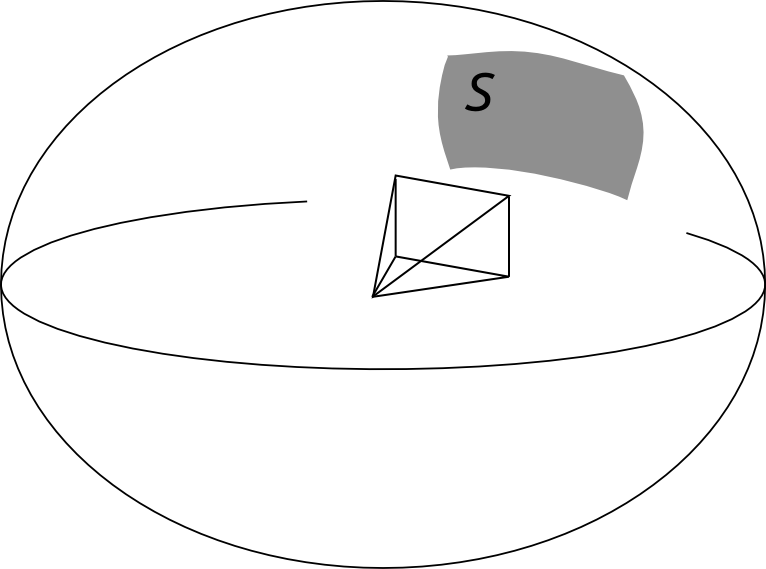
\includegraphics[width=0.6\textwidth]{Chapter3/graphics/calcul_density.png}
		\caption{Illustration du calcul de densité d'acquisition. La surface S correspond à la zone échantillonnée par le dispositif représenté, au sein de la sphère unité. Le calcul de l'angle solide est le ratio de ces deux surfaces}
		\label{fig:ch3_densité}
	\end{center}
\end{figure}

L'angle solide d'un dispositif de perception au sein de la sphère unité est potentiellement complexe, si la surface correspondante est quelconque. Il s'écrit formellement :
\begin{equation}
	\Omega = \int\limits_{S} \int \frac{ \vec{r} \cdot \vec{n} dS} {r^3}
\end{equation}
(avec $\vec{r}$ le vecteur entre le centre de la sphère et l'élément infinitésimal de surface intégré, et $\vec{n}$ le vecteur unité normal à la surface en ce point). Le calcul est simplifié pour les dispositifs que nous allons considérer par la suite, du fait de l'angle solide couvert, lorsqu'il s'agit d'un intervalle défini sur deux axes. En notant $\Delta_{\Phi}$ l'ouverture angulaire verticale, et $\Delta_{\Theta}$ l'ouverture angulaire horizontale, l'angle solide couvert s'écrit alors :

\begin{equation}
	\Omega = 4 \cdot \arcsin( \sin(\frac{\Delta_{\Phi}}{2}) \sin(\frac{\Delta_{\Theta}}{2}))
\end{equation}

Dans le cas d'un capteur ayant une couverture à $360^\circ$, l'angle solide $\Omega$ s'écrit :
\begin{equation}
	\Omega = 4 \Pi \cdot \sin(\frac{\Delta_{\Phi}}{2})
\end{equation}

\subsubsection{Comparaison selon les capteurs:}
Considérons maintenant quelques capteurs et usages typiques des tâches de perception (la densité est exprimée en nombre de points par millistéradians):

\begin{table}[H]
	\centerline {
		\begin{tabular}{|c | c| c | c | c | c |} 
			\hline
			\pbox{1cm}{Capteur\\ } & \pbox{8cm}{Nombre \\ de points} & \pbox{8cm}{Ouverture \\ verticale} & \pbox{8cm}{Ouverture \\ horizontale} & \pbox{8cm}{Angle \\ solide} & Densité (pt/msr) \\
			\hline
			Caméra - Épars 		& 100 	& 55$^\circ$		& 40$^\circ$ 	& 0.1 	& 1\\
			\hline
			Caméra - Épars 		& 4k 		& 55$^\circ$ 		& 40$^\circ$ 	& 0.1 	& 40\\
			\hline
			Caméra - Dense 		& 300k 	& 55$^\circ$ 		& 40$^\circ$	& 0.1 	& 3000\\	
			\hline
			Velodyne - HDL32 	& 128k 	& 26.8$^\circ$ 	& 360$^\circ$ & 0.5 	& 225\\	
			\hline
			Velodyne - HDL64 	& 256k 	& 26.8$^\circ$	& 360$^\circ$ & 0.5 	& 550\\ 
			\hline
			Kinect 						& 300k 	& 57$^\circ$ 		& 43$^\circ$ 	& 0.1 	& 2700\\ 
			\hline
			Radar 						& 125 	& 25$^\circ$ 		& 10$^\circ$ 	& 0.01 	& 10\\ 
			\hline
		\end{tabular}
	}
	\caption{Quelques exemples de densités d'échantillonnage}
	\label{tab:ch3_comp_densité}
\end{table}

On a choisi dans le tableau \ref{tab:ch3_comp_densité} une caméra de résolution 640x480 dans le cas d'un traitement dense, cette valeur pouvant être révisée à la hausse dans nombre de publications récentes, au prix de besoins accrus en termes de puissance de calcul (\cite{Lategahn2011}). Les valeurs de \emph{100} et \emph{4000} points choisis dans les algorithmes dits épars se veulent typiques de diverses implémentations de SLAM visuel, typiquement selon les approches par filtrage ou optimisation (cf. section \ref{sec:ch4_state_of_art}). Les ouvertures angulaires choisies dans le cas de la vision correspondent à un angle de vue \og standard\fg{} (d'une optique de focale 35mm dans le standard 24mm*36mm), et sont à moduler selon les installations expérimentales. Ces valeurs permettent de bien poser la problématique et les besoins en termes de suivi de points, dans le cadre de la vision. L'usage des lasers de type "Velodyne" est en effet courant dans les recherches sur l'automatisation des véhicules, et sa densité d'informations a prouvé être suffisante dans de nombreux usages urbains (Spinello et Siegwart \cite{Spinello2010}, Azim et Aycard \cite{Azim}, Mertz \textit{et al.} \cite{Mertz2013}). Elle nous servira donc de référence pour évaluer la pertinence d'une approche ponctuelle de la perception visuelle. Les caractéristiques des capteurs radar notamment utilisés dans l'automobile ont été repris de \cite{Schneider2006}.

\subsubsection{Quelques remarques:}
On pourra, par exemple, distinguer les points suivants :
\begin{itemize}
	\item On compare dans le tableau \ref{tab:ch3_comp_densité} des densités d'échantillonnage entre un capteur télémétrique à balayage et un système de vision, sans tenir compte des limites de ces derniers, qui peuvent diminuer l'échantillonnage effectif. En pratique de nombreux facteurs peuvent impacter la qualité de la perception visuelle, notamment : \\
	
		\begin{itemize} \renewcommand{\labelitemii}{$\cdot$}
			\item{\emph{les conditions d'illumination:\\}}
			La dynamique d'un capteur d'imagerie étant communément limitée à environ 12 bits, les parties de l'image dont l'éclairement relatif à l'éclairement moyen est au delà de cette dynamique maximale seront perçues comme uniformes, aucun point ne pouvant alors être suivi. Un exemple en est présenté sur la figure \ref{fig:ch3_saturated_pic}, sur laquelle un histogramme de la luminosité des pixels permet de mettre en évidence une saturation de l'acquisition dans les tons clairs.\\
			
			\item{\emph{la dynamique du porteur ou des éléments mobiles:\\}}
			Dans le cas d'un mouvement trop rapide, la vitesse d'obturation peut ne pas être suffisante pour rendre négligeable le mouvement perçu pendant le temps d'intégration. L'objet imagé est dans ce cas mal défini, jusqu'à éventuellement compromettre la possibilité même d'un suivi de points caractéristiques dans le temps. Cette mauvaise définition peut également avoir un impact sur la détection de points d'intérêt, comme présenté dans \cite{Mei2010}.\\
			
			\item{\emph{la "détectabilité" propre des objets:\\}}
			Le traitement des informations visuelles est sensible (quelque soit la solution technique retenue) à l'aspect des objets, et peut notamment être mis en défaut par des objets parfaitement uniformes.\\
		\end{itemize}

	\item L'utilisation simultanée d'un nombre raisonnable de caméras (6 caméras par exemple, si tant est que la puissance de calcul nécessaire soit disponible, et que les critères précédents soient remplis) permet de couvrir un angle solide équivalent aux capteurs de type \og Velodyne\fg{}. C'est une approche retenue par Meilland \textit{et al.} (\cite{Meilland2011}) par exemple.\\
	
	\item On ne parle ici que d'une mesure possible pour évaluer la quantité d'un type d'informations perçues, pas nécessairement de l'ensemble des informations que l'état de l'art parvient à en extraire. De très nombreuses applications sont ainsi disponibles pour exploiter des images, ou des nuages de points. Il s'agit donc d'une base de comparaison arbitraire, en aucun cas exhaustive.
\end{itemize}

\begin{figure}
	\begin{center}
		\begin{subfigure}{0.48\textwidth}
			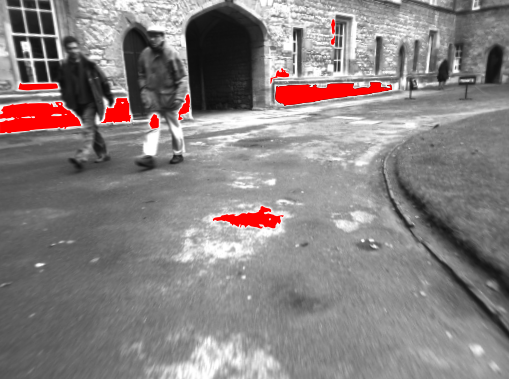
\includegraphics[width=\textwidth]{Chapter3/graphics/NewCollege_overexposed.png} 
		\end{subfigure}
		~
		\begin{subfigure}{0.48\textwidth}
			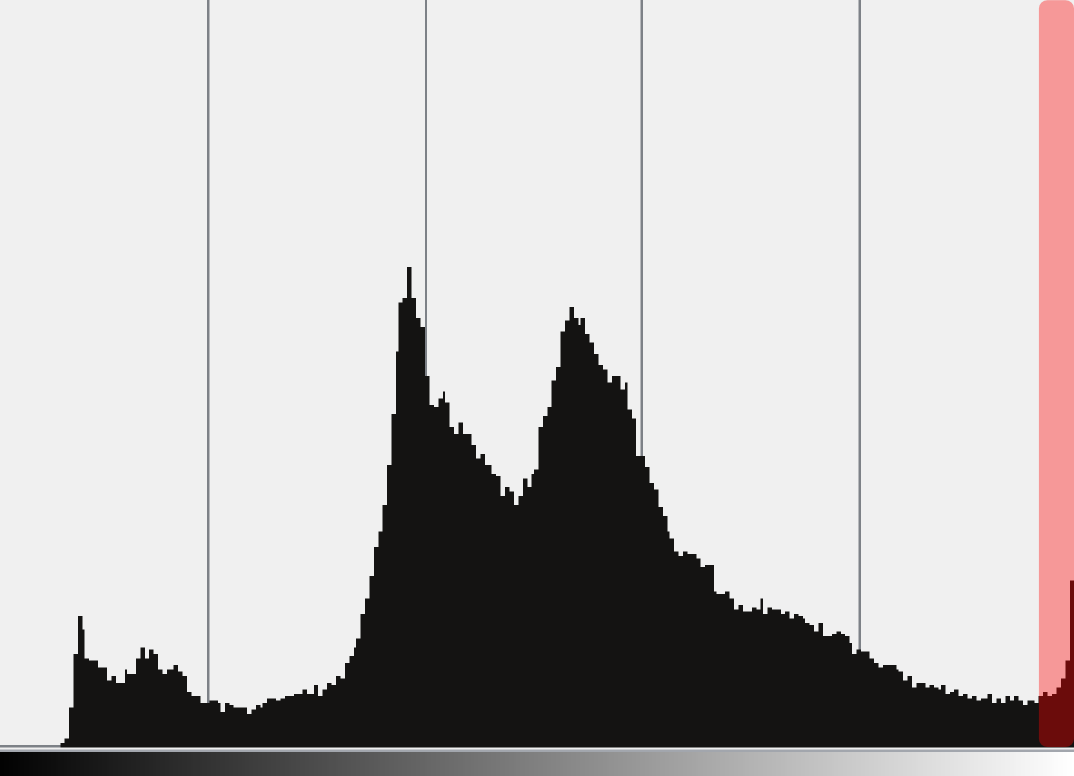
\includegraphics[width=\textwidth]{Chapter3/graphics/NewCollege_histogram_red.png} 
		\end{subfigure}
		
		\caption{Illustration de la saturation possible du capteur d'imagerie. Un histogramme de la répartition des valeurs de niveaux de gris des pixels est représenté, la saturation étant visible de part une accumulation des valeurs extrêmes de l'histogramme. Les zones saturées sont représentées en rouge sur l'image, et correspondent à l'accumulation sur la droite de l'histogramme des valeurs de luminosité}	
		\label{fig:ch3_saturated_pic}
	\end{center}
\end{figure}

\subsection{Algorithmes \og épars\fg{}} \label{sec:ch3_Vision_epars}
Cette partie est consacrée aux algorithmes basés sur un suivi de points singuliers, par opposition aux suivis denses (\ref{sec:ch3_Flux_optique_dense}) qui sont par ailleurs de plus en plus populaires dans la littérature. On pourrait tout d'abord se demander pourquoi une telle approche est-elle seulement nécessaire, puisque le suivi de l'ensemble des points est possible ? Différents arguments sont possibles, on citera notamment les critères de qualité du suivi de points, primordiale dans notre approche, ainsi que les contraintes de temps de calcul. 

\subsubsection{Sélection des points d'intérêt:} \label{sec:ch3_Détection_points_intérêt}
Dans le cas où tous les points d'un image ne sont pas considérés, il semble important d'en assurer une sélection pertinente en préalable à toute opération. Tous les points d'une image n'ont en effet pas la même valeur selon les usages, mais plusieurs critères sont possibles. En règle générale, les points indistinguables de leur voisins ont une contribution très faible à l'information portée par l'image (par exemple dans le cas d'une zone contiguë dans laquelle la réponse du capteur est saturée), et l'on peut raisonnablement supposer qu'ils n'auront jamais d'intérêt à être mis en avant. En revanche, la sélection des points "<principaux\fg{} parmi ceux restant n'est pas simple, et pourrait être envisagée selon deux aspects : qualité intrinsèque des points au sein de l'image, et leur adéquation à l'usage visé. Schmid et al. (\cite{Schmid2000}) proposent ainsi deux critères pour la sélection de points : la quantité d'information présente (liée au degré d'entropie locale) et la répétabilité, considérant donc par ce deuxième critère que l'usage qu'il est fait des points détectés (par exemple SLAM, ou suivi d'objet) rentre aussi en compte. Il s'agit de l'approche que nous avons suivi dans notre comparaison de trois détecteurs (\ref{sec:ch3_Eval_PI}), prenant en compte le temps de calcul nécessaire à la détection d'un nombre de points donnés, et la qualité de ceux-ci dans une perspective de suivi dans le temps.\\

La détection de points d'intérêts présente dans la littérature s'articule autour de trois grandes approches, que l'on peut résumer brièvement par les quantités suivantes: 
\begin{itemize}
	\item{\emph{Contour:\\}} 
	les points d'intérêt se situent sur des points remarquables des contours détectés dans l'image. \\

	\item{\emph{Intensité:\\}}
	les valeurs d'intensité sur un voisinage sont discriminantes, par exemple la réponse à une fonction d'auto-corrélation.\\

	\item{\emph{Optimisation paramétrique:\\}}
	on pré-suppose une forme arbitraire pour les points recherchés, cette forme définit une fonction de coût dont les extrema sont recherchés dans l'image.\\
\end{itemize} 

On présente dans la suite quelques uns des détecteurs de points d'intérêt les plus utilisés, mais cet état de l'art ne peut être exhaustif dans le cadre de ce manuscrit de thèse, et le lecteur pourra se reporter sur la littérature du domaine pour plus d'informations (par exemple \cite{Tuytelaars2007} et \cite{Schmid2000} pour une revue, \cite{Shi2002} \cite{Bay} \cite{Lowe1999a} et \cite{Rosten} pour des articles de référence, ou encore \cite{Sood2008} pour une application au SLAM visuel). 

\paragraph{Harris:\\}
Le détecteur de Harris s'intéresse aux points singuliers en terme de gradient, et considère pour cela une fonction de coût, basée sur l'intensité des pixels sur un voisinage donné. Celle-ci exploite une proposition de Moravec (\cite{Moravec1980}), qui propose en 1980 de considérer la somme des différences au carré (\emph{Sum of Squared Differences}, souvent noté SSD) autour du point considéré. Harris (\cite{Harris1988}) introduit en 1988 une approximation de la dérivée seconde de cette fonction de coût, en utilisant la matrice Hessienne :
\begin{equation} \label{eq:ch3_Harris_H}
	H_{Harris} = \left[ 
		\begin{array}{cc}
		\widehat{I_x}^2 & \widehat{I_x} \widehat{I_y} \\
		\widehat{I_x} \widehat{I_y} & \widehat{I_y}^2  
		\end{array} 
	\right]
\end{equation}
avec $\widehat{I_x}$ un opérateur réalisant la différence des valeurs d'intensités sur un voisinage selon l'axe $x$. La réponse du détecteur est alors, avec $k$ un paramètre d'ajustement :
\begin{align}
	R &= Det(H) - k*Tr(H)^2
	k &= \textnormal{paramètre d'ajustement}
\end{align}

Cette réponse dépend de l'amplitude des valeurs propres de la matrice $H$, sans pour autant en nécessiter le calcul explicite. Ce détecteur peut se montrer trop sensible au bruit présent dans l'image, auquel cas un lissage peut être initialement appliqué. Il est également possible de choisir la fonction de différence $I$ pour mieux prendre en compte ce problème. Un défaut de ce détecteur, développé dans la suite de notre étude, est en outre sa sensibilité à des forts gradients unidimensionnels. Celle-ci peut l'amener à sélectionner des points dont l'unicité sur un voisinage proche n'est pas garantie.

\paragraph{Shi et Tomasi : "Good Features To Track"\\}
Ce détecteur a été présenté dans \cite{Shi2002}, et se base sur le détecteur précédent. Dans cet article, Shi et Tomasi ont réalisé une étude très complète de cas pratiques de suivi d'éléments d'une scène, en considérant notamment les altérations visibles entre le même élément physique imagé de plusieurs points de vue. Leur étude portant sur des transformation affine des images les amène à recommander l'usage des valeurs propres  $\lambda_1$ et $\lambda_2$ les plus faibles de l'équation \ref{eq:ch3_Harris_H} comme fonction de coût, soit :
\begin{equation}
	R = min(\lambda_1, \lambda_2)
\end{equation}

\paragraph{\emph{SIFT} (Scale Invariant Feature Transform):\\}
Cet algorithme a été proposé par Lowe et al. (\cite{Lowe1999a}), et comprend une étape de détection et une étape d'extraction de descripteur, c'est-à-dire une signature caractéristique et répétable d'un élément de l'image, qui peut permettre de le retrouver sur une autre prise de vue. Nous ne nous intéresserons qu'à la détection de points d'intérêt de part notre approche, et le descripteur SIFT (qui signifie Scale Invariant Feature Transform) ne sera pas utilisé.\\
La procédure retenue pour la détection de points SIFT passe par la réalisation d'une pyramide d'images, obtenues par une convolution de l'image originale avec un noyau gaussien suivie d'un sous-échantillonnage. Le nombre d'étages de la pyramide d'image est l'un des paramètres de l'algorithme. Chaque étage contient plusieurs versions de l'image à la même échelle, ayant subit un nombre plus ou moins important de convolutions par un noyau gaussien. Ceci permet ensuite d'utiliser la fonction \og Différence de Gaussiennes\fg{}, en soustrayant à une image de référence une image plus convoluée, les points d'intérêt SIFT étant alors recherchés parmi les extrema locaux de cette fonction. On pourra remarquer que les points obtenus sont alors théoriquement invariants d'échelle, la convolution par un noyau gaussien étant par ailleurs l'un des moyens les plus appropriés de mise à l'échelle d'une image (\cite{Lindeberg1994}). La recherche de points SIFT peut donc se résumer à la recherche de points saillants dans l'espace des différentes échelles de l'image. Cette recherche commence par l'échelle la plus basse, seuls les points saillants d'une échelle donnée sont ensuite recherché à l'étape supérieure. Une illustration de cet algorithme est visible sur la figure \ref{fig:ch3_SIFT}.

\begin{figure}
	\centerline{
		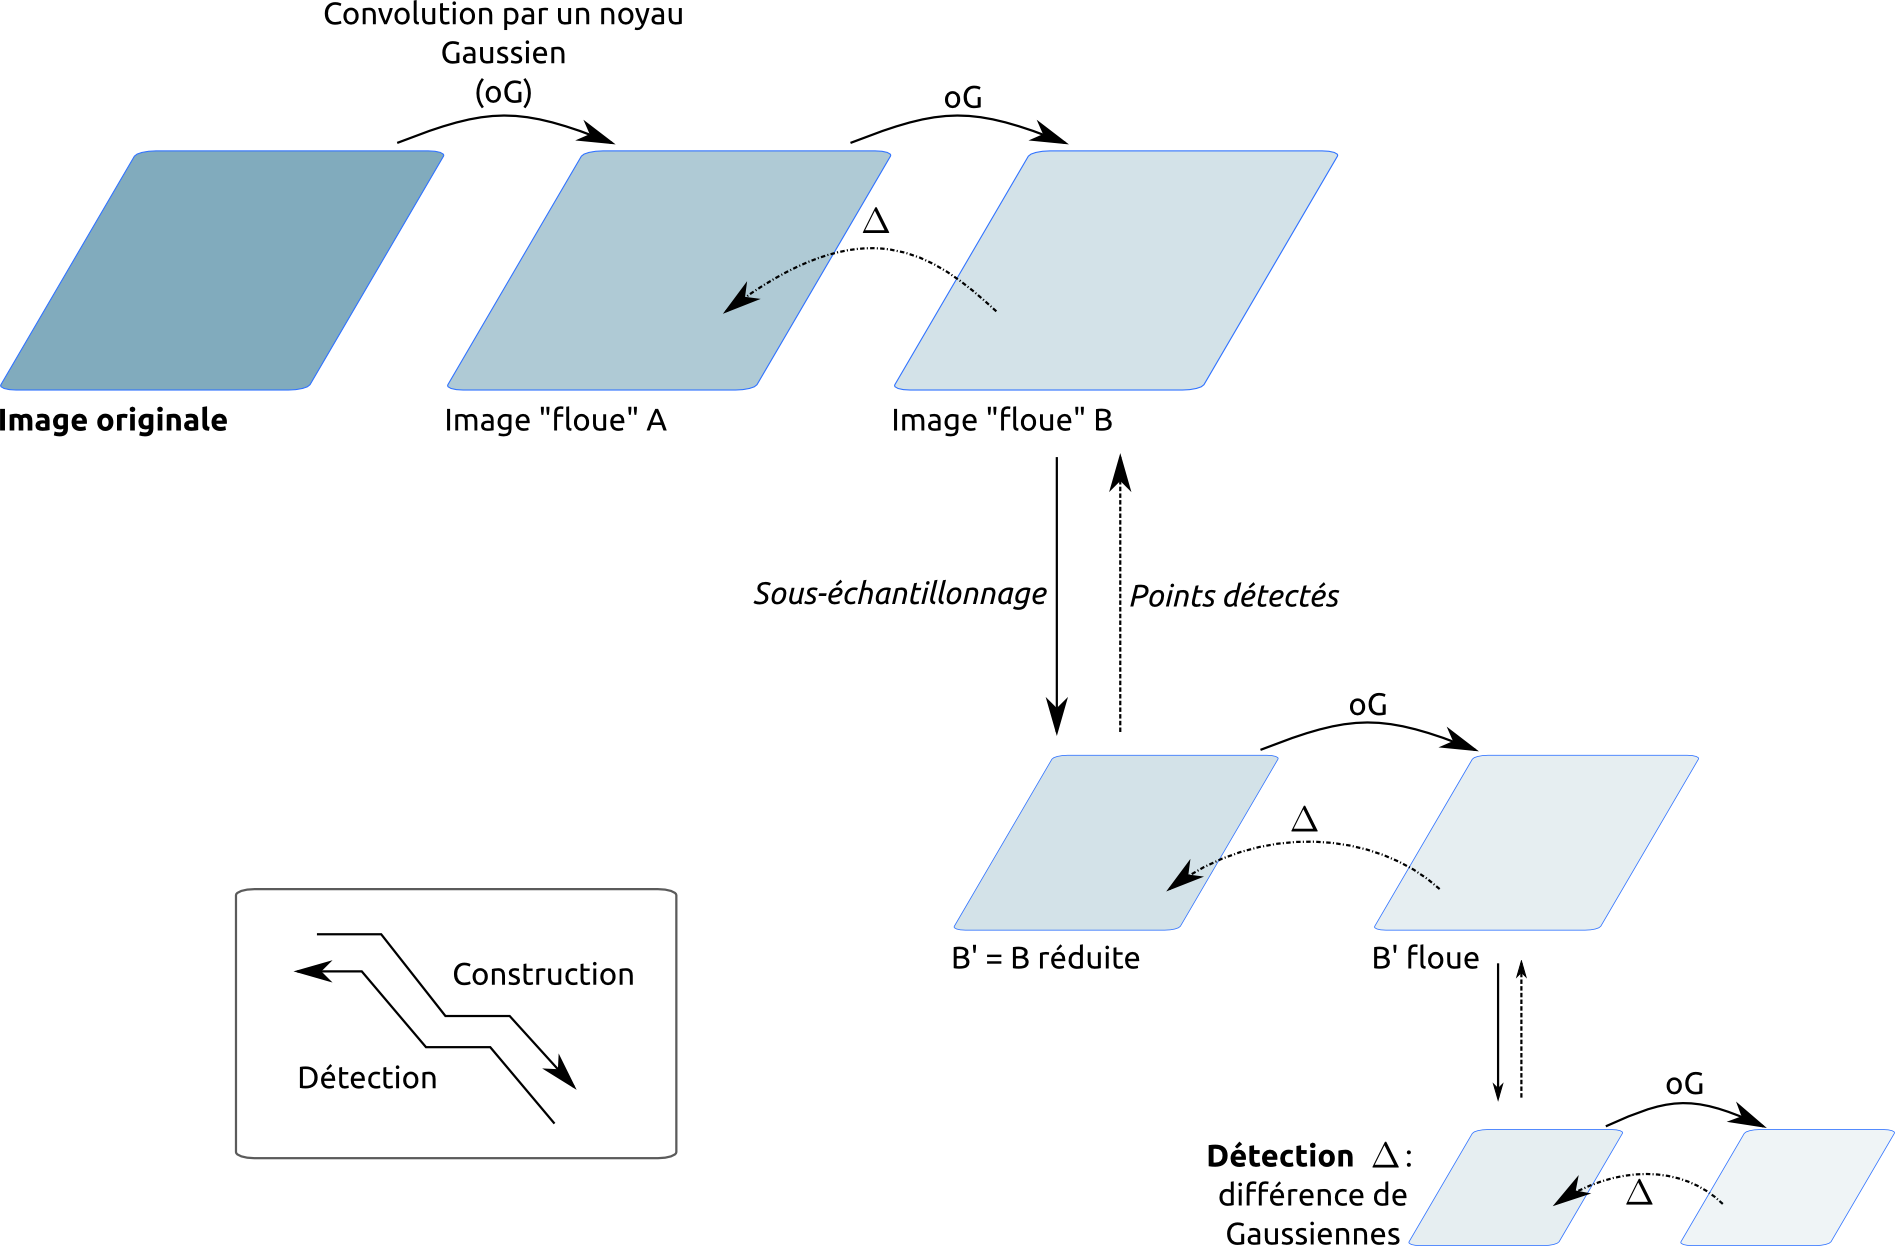
\includegraphics[width=0.9\textwidth]{Chapter3/graphics/SIFT.png}
		}
	\caption{Schéma de fonctionnement de l'algorithme SIFT}
	\label{fig:ch3_SIFT}
\end{figure}

\paragraph{\emph{SURF} (Speeded Up Robust Feature):\\}
Cet algorithme, présenté par Bay et al. dans \cite{Bay}, désigne lui aussi à la fois un détecteur de points d'intérêt et un descripteur. Nous ne nous intéresserons qu'à la détection de points d'intérêt dans cette partie, et ne ferons donc pas une description complète de SURF. \\
Bay propose de se baser sur la matrice hessienne de l'intensité, c'est-à-dire la matrice des dérivées partielles secondes de la fonction intensité. Il propose par ailleurs que cette matrice hessienne soit appliquée sur une image convoluée par une Gaussienne, et non l'image originale, la convolution par une gaussienne permettant une mise à l'échelle de l'image (et l'invariance du détecteur à celle-ci).

\begin{equation} \label{SURF_H}
	H_{SURF} = \left[ 
		\begin{array}{cc}
		L_{xx}(x, \sigma) & L_{xy}(x, \sigma) \\
		L_{xy}(x, \sigma) & L_{yy}(x, \sigma)  
		\end{array} 
	\right]
\end{equation}
avec $L_{xx}(x, \sigma)$ désignant la convolution de la dérivée seconde d'une gaussienne $\frac{\partial^2 g(x, \sigma)}{{\partial x}^2}$ avec l'image au point $P(x,y)$. \\

Bay  et al. proposent par ailleurs une approximation de cette matrice, suivant en cela un procédé similaire à la construction des points SIFT (\cite{Lowe1999a}), qui rend  $L_{xx}(x, \sigma)$ discrète et simplifie fortement son calcul. On note cette approximation $D_{xx}$ par la suite, comme proposé dans \cite{Bay}. Ce calcul est enfin réalisé par le biais d'une \emph{image intégrale} (procédé courant en traitement d'image consistant à enregistrer pour chaque pixel la valeur cumulée des pixels précédents) de l'application sur l'image complète de $D_{xx}$ ,  $D_{xy}$  et $D_{yy}$. Ce procédé permet de calculer les dérivées nécessaires sur l'intégralité de l'image, puis de calculer la valeur du détecteur en un point $P(x,y)$ par soustraction des valeurs voisines de l'image intégrale, ce qui minimise les calculs redondants lors d'une détection de points d'intérêt sur une image donnée.\\

La fonction de coût conduisant à la détection ou non d'un point d'intérêt est finalement une approximation du déterminant de H (équation \ref{SURF_H}), dont la justification est visible dans \cite{Bay} (le coefficient 0.9 visant à pondérer l'erreur faite dans le calcul de déterminant par la discrétisation):
\begin{equation} \label{eq:ch3_SURF_R}
	R = D_{xx} * D_{yy} - (0.9 * D_{xy})^2
\end{equation}
Un point d'intérêt est finalement sélectionné dès que la réponse $R$ du détecteur SURF (équation \ref{eq:ch3_SURF_R}) dépasse un seuil préalablement fixé.

\paragraph{\emph{FAST} (Features from Accelerated Segment Test):\\}
Le détecteur de points d'intérêt \emph{FAST} (Rosten et al. ,\cite{Rosten}) a été obtenu par apprentissage, et diffère en cela des définitions \og déterministes\fg{} des points Harris et SURF. Il se base cependant sur une observation \emph{a priori}, celle d'une recherche de points d'intérêts sous la forme de \og coins\fg{} contrastés. Cette recherche se fait en parcourant un cercle dit de Bresenham (discrétisé sur la matrice des pixels), comme initialement proposé dans \cite{Rosten2005}. Un coin se caractérise alors par un segment continu sur ce cercle de valeur relativement homogène, et nettement inférieure (ou supérieure) à celle du pixel central $P$, comme l'illustre la figure \ref{fig:ch3_FAST_illustration}.\\

Cette définition doit être testée sur l'ensemble des segments obtenus en parcourant le cercle de Bresenham pour valider l'existence ou non d'un \og coin\fg{} en son milieu. Chacun de ces tests constitue alors le nœud d'un arbre binaire, qui sera parcouru tant que le test précédent est positif. Cette structure permet donc un rejet rapide des  mauvais candidats, sans avoir nécessairement à effectuer l'ensemble des calculs nécessaires sur un voisinage, comme il est l'usage pour d'autres détecteurs. Cette caractéristique est intéressante en pratique, les points d'intérêt étant empiriquement très minoritaires dans une image. Rosten et al. proposent d'optimiser par apprentissage l'organisation de cet arbre de décision, afin que les réjections les plus probables soient effectuées plus avant, et évitent des calculs probablement inutiles. Cette optimisation a été réalisée dans le cas du détecteur \emph{FAST} par un réseau de neurones, et conduit à l'arbre binaire statique qui est maintenant couramment utilisé dans d'autres travaux (voir par exemple BRIEF, par Calonder et al. \cite{Calonder2010}, ou FREAK, par Alahi \cite{Alahi}).

\begin{figure}
	\centering{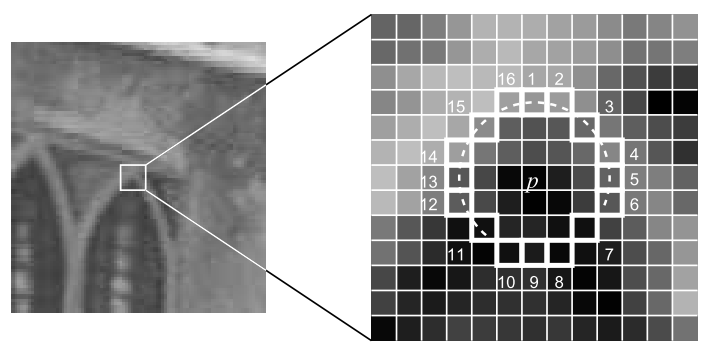
\includegraphics[width=0.68\textwidth]{Chapter3/graphics/FAST.png}}
	\caption{Une illustration partielle du détecteur FAST (source : Rosten\textit{ et al.} \cite{Rosten}). Les pixels surlignés de blanc représentent les extrémités des segments testés à partir du pixel central pour infirmer ou confirmer sa singularité.}
	\label{fig:ch3_FAST_illustration}
\end{figure}

\subsubsection{Suivi de points} \label{sec:ch3_suivi_de_points}
\paragraph{Par re-détection de points d'intérêt:\\}
Une première méthode consiste à utiliser la détection de points d'intérêt pour les images sur lesquelles le suivi doit être assuré, puis une mesure de similarité entre le point d'intérêt initial et les points d'intérêts détectés dans un voisinage donné sur la seconde image. Il s'agit par exemple de l'approche suivie par Davison dans le domaine du SLAM visuel (\cite{Davison2003}), ou plus récemment par Clipp, Nistér ou Mei par exemple (\cite{Clipp, Nister2006, Mei2010}). La détection peut dans ce cas se faire à l'aide des algorithmes présentés dans \ref{sec:ch3_Détection_points_intérêt}, tandis que la mesure de similarité peut prendre différentes formes, par exemple \textit{SSD} (\emph{Sum of Squared Differences}, somme des différences au carré) ou \textit{SAD} (\emph{Sum of Absolute Differences}, somme des différences absolues) ; normalisés par une soustraction de leurs valeurs moyennes en intensité pour rendre ce suivi plus robuste aux changements d'illumination.

%Mettant l'accent sur le suivi de points sur le plus grand nombre d'acquisitions possible, nous n'avons pas retenu cette approche, du fait du risque de disparition d'un point d'intérêt au fur et à mesure d'un changement de perspective, par exemple. Une autre méthode consiste à rechercher par optimisation la position d'un point sur une nouvelle image, sans supposer que celui-ci soit de nouveau détectable en tant que point d'intérêt prédominant.

\paragraph{Par optimisation itérative:\\}
Le suivi de points d'intérêt peut également prendre une autre forme, consistant à cherche l'optimum d'une fonction de vraisemblance autour de la position initiale du point d'intérêt. L'algorithme de référence dans cette approche a initialement été introduit par Lucas et Kanade (\cite{Lucas1981a}) sous la forme d'une descente de gradient, puis perfectionné par un algorithme pyramidal le rendant plus apte à suivre des mouvements importants par Bouguet (\cite{Bouguet2001a}). Cet algorithme suppose que l'illumination de l'image reste constante, mais cette condition peut éventuellement être relâchée par une adaptation de l'illumination moyenne (\cite{Zach2008}). \\

Cet algorithme est détaillé en annexe (\ref{sec:Annexe_klt}), mais nous pouvons d'ores et déjà remarquer qu'il s'agit d'une approche locale, pouvant relativement aisément être mise en défaut. On peut par exemple imaginer le cas du suivi d'un élément d'un motif répétitif, pour lequel de nombreux optimum locaux vont exister. Par ailleurs, cet algorithme suppose de descendre un gradient local pour ajuster la position recherchée, ce qui suppose donc qu'il soit bien défini. D'autres techniques d'optimisation sont possibles, prenant en compte une optimisation globale. On pourra citer une approche par Graph Cut (\cite{Freedman}, \cite{Boykov}, ou bien l'application \emph{a posteriori} de contraintes de régularité, qui nécessitent dans ce cas le calcul quasi-dense du flux optique (voir \ref{sec:ch3_Flux_optique_dense}).


\subsection{Algorithmes denses}\label{sec:ch3_Flux_optique_dense}
Le suivi de points peut également être réalisé de manière dense, c'est-à-dire que tous les points de l'image sont alors mis à contribution. Les méthodes présentées dans la section \ref{sec:ch3_suivi_de_points} sont évidemment généralisables, mais cette utilisation n'est le plus souvent pas souhaitable. Les suivis de points proposés consistent en effet en une optimisation locale, qui ne prend pas en compte la cohérence globale du suivi des points. Cette approche peut être mise en défaut lors du suivi de zones uniformes de l'image, pour lesquels les différents points de convergence de ces algorithmes locaux ne conserveront \textit{a priori} pas la contrainte de quasi-uniformité. Elle peut également être mise en défaut sur les zones bien définies et non-uniformes, mais pour lesquelles une répétition de motif propose plusieurs \og attracteurs\fg{} (suivi de points sur un damier par exemple). Les méthodes itératives (KLT) ou par re-détection peuvent dans ce cas converger vers un minimum local dépourvu de réalité physique. \\
Pour toutes ces raisons, de nombreuses contributions alternatives ont été proposées pour résoudre le problème du suivi dense de points dans une image, également appelé flux optique. Une étude approfondie serait hors de propos dans le cadre de ce manuscrit, mais on pourra en présenter quelques méthodes parmi les plus reconnues:

\paragraph{\emph{Horn-Schunk}:\\}
Cette technique fut initialement proposée dans \cite{Horn1981}, et se base sur une équation contraignant les changements de luminosité avec le mouvement perçu d'une partie de l'image. De fait, en supposant que la luminosité de chacun des éléments de la scène est inchangée, on constate aisément que le flux optique (le vecteur vélocité des déplacements perçus des éléments de l'image) doit alors être perpendiculaire au gradient de luminosité. Cette contrainte n'est cependant pas suffisante, car elle ne permet notamment pas la détermination du mouvement le long des lignes d'égale luminosité, et d'autres éléments sont donc nécessaires. \\
Supposant que le flux optique le long d'éléments homogènes de la scène devra être lui aussi homogène, Horn et Schunck (\cite{Horn1981}) proposent de prendre également en compte une contrainte de lissage, définie comme le carré du gradient de la vélocité : ${\frac{\partial{u}}{\partial{x}}}^2 + {\frac{\partial{u}}{\partial{y}}}^2$ et  ${\frac{\partial{v}}{\partial{x}}}^2 + {\frac{\partial{v}}{\partial{y}}}^2$ (avec $u$ et $v$ les deux composantes du déplacement sur l'image). La méthode de Horn et Schunk consiste alors à trouver le champ de vitesse $(u,v)$ minimisant les erreur cumulées de changement de la luminosité et du carré du gradient de la vélocité. En notant, comme dans l'article fondateur de Horn et Schunk, $E(x,y,t)$ la luminosité d'un point $P(x,y)$ de l'image au temps $t$, l'erreur $\Delta E$ que l'on cherche à minimiser sur chacun des pixels s'écrit, avec $\Lambda$ la contrainte de lissage que l'on fixe par ailleurs :\\

\begin{align}
	{\Delta E}_{Ill.}^2 &= 	\left( \frac{\partial E}{\partial x} \cdot u + \frac{\partial E}{\partial y} \cdot v + \frac{\partial E}{\partial t} \right)^2 \\
	{\Delta E}_{Cont.}^2 &= {\frac{\partial{u}}{\partial{x}}}^2 + {\frac{\partial{u}}{\partial{y}}}^2 \\
	{\Delta E}^2 &= 				{\Delta E}_{Ill.}^2 + \Lambda \cdot {\Delta E}_{Cont.}^2
\end{align}

Horn et Schunk montrent par ailleurs que le coefficient $\Lambda$ doit être de l'ordre de l'erreur attendue dans la détermination du vecteur de déplacement dans l'image.

\paragraph{\emph{Tenseur d'orientation}:\\}
Proposée initialement par G. Farneback (\cite{Farneback2000} puis \cite{Farneback}), cette méthode exploite une représentation en trois dimensions de l'évolution du vecteur vélocité $u$ dans le temps, sous la forme d'une matrice tensorielle, symétrique semi-définie et positive $T$. Cette matrice décrit l'évolution de la luminosité localement selon trois dimensions (espace et temps), de sorte que le vecteur vélocité peut en être déduit comme son vecteur propre associé à la valeur propre 0 (on suppose que la vélocité est conservée sur un même élément source). Farneback propose donc un mécanisme permettant de calculer l'ensemble des matrices $T$ de manière efficace, ainsi qu'une minimisation de ${u}^T T u$ conduisant à une estimation robuste du vecteur vitesse $\hat{u}$. Un exemple exploitant cette méthode est visible sur la figure \ref{fig:ch3_OF_Farneback}.\\

\begin{figure}
	\begin{subfigure}{0.48\textwidth}
		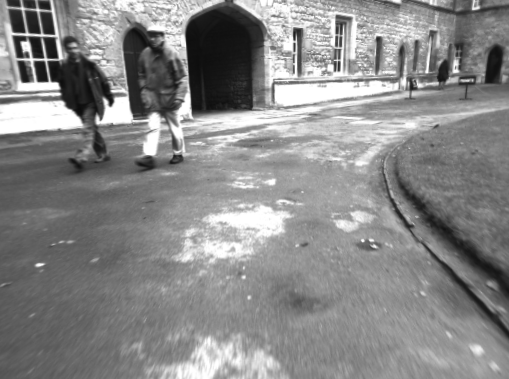
\includegraphics[width=\textwidth]{Chapter3/graphics/OF_Farneback_RAW.png} 
	\end{subfigure}
	~
	\begin{subfigure}{0.48\textwidth}
		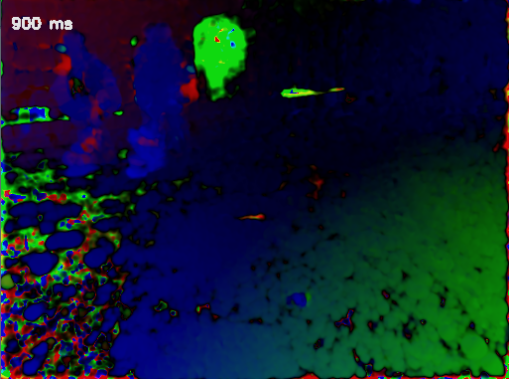
\includegraphics[width=\textwidth]{Chapter3/graphics/OF_Farneback.png}
	\end{subfigure}
	
	\caption{Flux optique dense : méthode de Farneback (implémentation OpenCV). Le code couleur utilisé pour signaler la direction des vecteurs de déplacement est précisé sur la figure \ref{fig:ch3_code_couleur}}
	\label{fig:ch3_OF_Farneback}
\end{figure}

\paragraph{\emph{Graph Cut}:\\}
Les méthodes dites de \emph{Graph Cut} représentent l'espace des solutions possibles comme un graphe, la solution optimale étant alors une section de celui-ci minimisant une fonction de coût. La définition de cette dernière rend possible la prise en compte de contraintes globales dans la recherche d'une solution, le résultat étant très dépendant des paramètres pris en compte. Freedman et al. (\cite{Freedman}) proposent par exemple la détermination du changement global d'illumination a priori, conservant dans la procédure de \og graph cut\fg{} les coûts (ou l'énergie, les formulations peuvent différer) liés à un changement local de luminosité.

D'autres approches sont par ailleurs possibles, notamment en combinant des méthodes locales et globales de calcul du flux optique (par exemple \cite{Bruhn2005} qui combine Horn-Schunk et KLT). Nous n'avons pas retenu ces méthodes pour deux raisons : leur coût en termes de calcul est très important, et les contraintes apportées, si elles permettent le lissage des point aberrants, n'apportent pas réellement d'information supplémentaire. En effet, hors implémentation très agressive et difficilement généralisable dans le domaine de la robotique (\cite{Dumortier} par exemple pour un calcul intégralement sur GPU), le suivi de point dense est encore loin d'être temps réel. Par ailleurs, les différentes contraintes présentées dans les méthodes précédentes permettent d'obtenir une solution globalement améliorée par rapport à une optimisation naïve, mais elles n'offrent aucune garantie d'améliorer les résultats locaux. On constate ainsi aisément sur la figure \ref{fig:ch3_OF_Farneback} que de nombreuses zones de l'image ne sont pas correctement suivies, sans que cette information ne soit immédiatement accessible (certains algorithmes proposent cependant une évaluation intrinsèque de la qualité du suivi). Nous avons finalement choisi de nous concentrer sur le suivi de points saillants, aussi nombreux que possible, mais non denses. Un mécanisme de rejet, obtenu par le cumul de quatre suivis non-corrélés, nous permet enfin de ne conserver que les points fiables.

\section{Algorithme proposé} \label{sec:ch3_Vision_mécanisme}
\subsection{Processus général : Détection et maintien d'un ensemble de points d'intérêt}
Le processus proposé pour l'acquisition des indices visuels, illustré sur la figure \ref{fig:ch3_processus} est superficiellement présenté dans les points suivants. Nous détaillerons ces éléments dans les sections suivantes, on ne présente ici que les principes retenus : \\
\begin{itemize} \renewcommand{\labelitemii}{$\cdot$}
	\item \textbf{Initialisation:} \\ 
	Recherche de points d'intérêt	\\
	
	\item \textbf{Itérations:}
	\begin{enumerate}
		\item Suivi redondant des points sur une paire stéréo
		\item Recherche des points aberrants
		\item Sélection de nouveaux points dans l'image courante:
		\subitem - utilisation d'un masque pour éviter l'accumulation de points sur les zones texturées
		\subitem - tri des meilleurs points obtenus
		\subitem - pression de sélection pour augmenter les points sur une zone privilégiée
	\end{enumerate}
\end{itemize}

\begin{figure}[h]
	\centering
	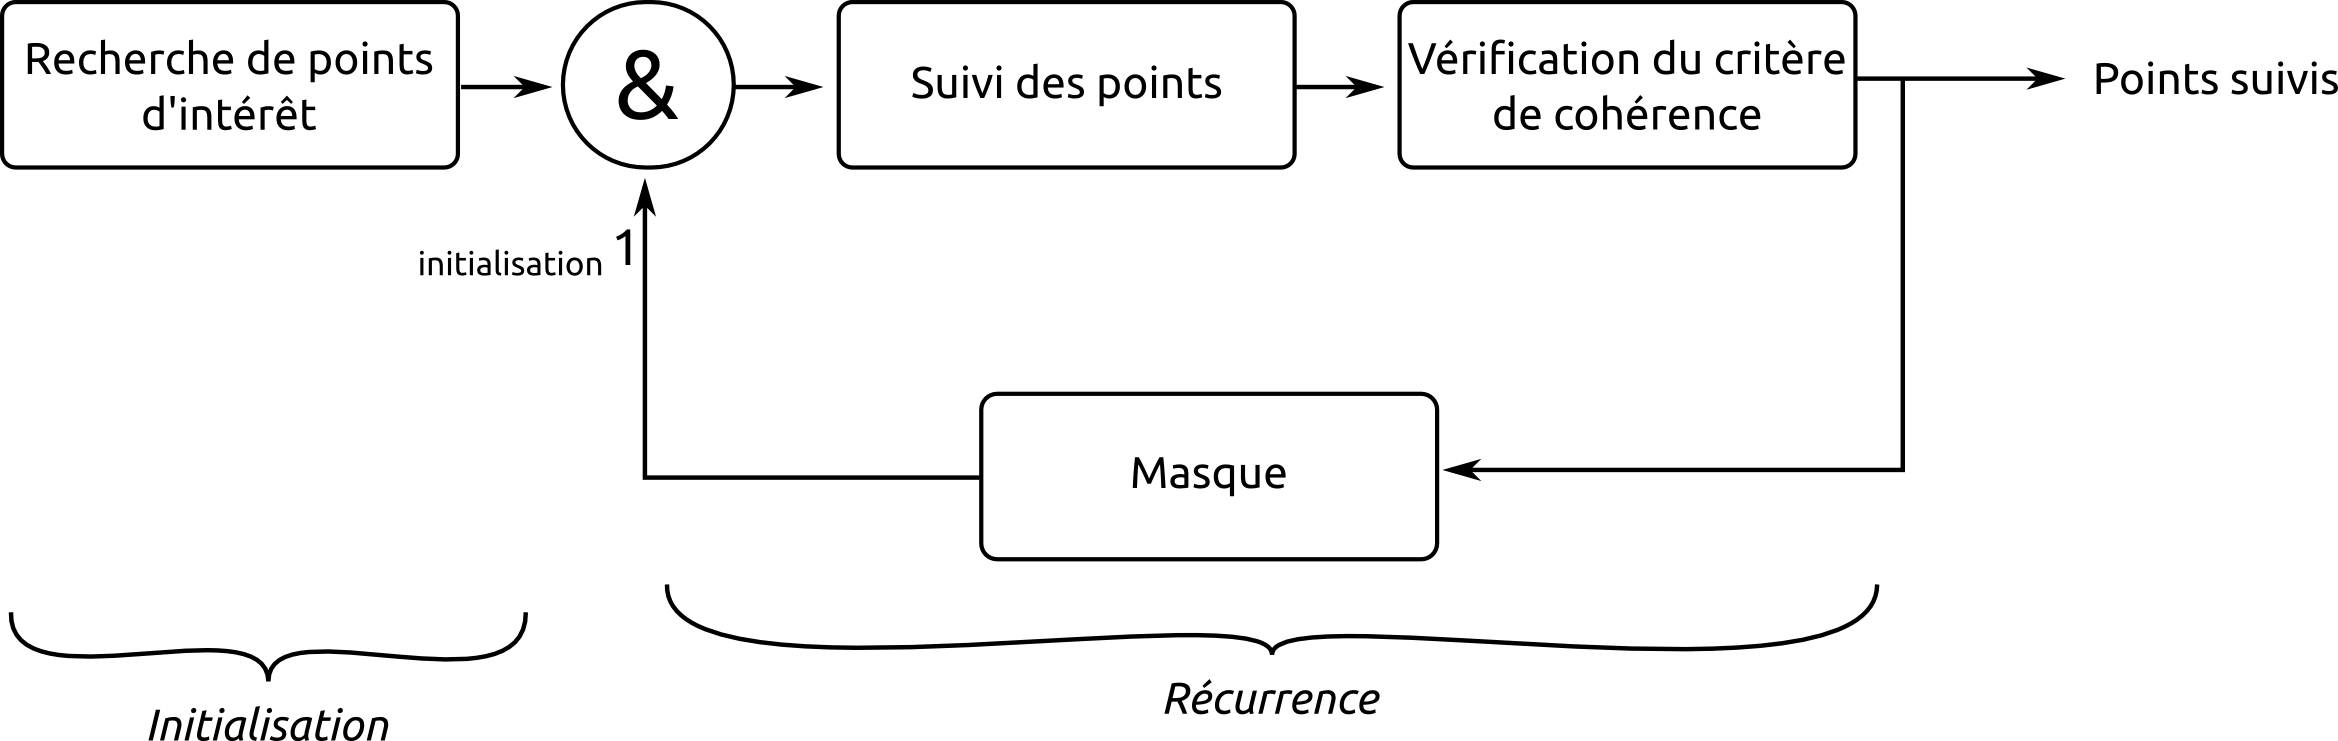
\includegraphics[width=0.9\textwidth]{Chapter3/graphics/tracking_process.png}
	\caption{Processus proposé pour maintenir un ensemble de points suivis}
	\label{fig:ch3_processus}
\end{figure}

Cet algorithme s'applique sur des paires d'images, la vérification de la fiabilité du suivi de points étant réalisée par redondance grâce à un suivi sur des paires d'images et dans le temps. Il vise à maintenir à chaque nouvelle acquisition un ensemble de points suivis représentatifs de l'environnement, et dont la fiabilité est raisonnablement garantie. Des points sont nécessairement perdus lors de chaque nouvelle acquisition, du fait du déplacement du porteur et de la modification de son champ de vision, ce qui rend le processus de ré-introduction de points obligatoire, quel que soit l'algorithme de suivi de points. \\
On essaie de garantir la représentativité de cet ensemble de points selon deux critères : la densité des points doit être localement uniforme, tandis que certaines zones définies comme d'intérêt peuvent être favorisées par rapport à d'autres. On souhaite ainsi être capable de s'affranchir des disparités locales de texture et de contraste, tout en étant capables si besoin d'augmenter la densité locale d'échantillonnage sur les zones perçues comme importantes. 

\subsection{Choix d'un algorithme de suivi de points}
On peut tout d'abord détailler le choix de l'algorithme de suivi de points, parmi les techniques proposées dans la section \ref{sec:ch3_suivi_de_points}.  Comme nous aurons l'occasion de le détailler par la suite, l'un des enjeux de notre méthode consiste à exploiter l'accumulation des observations pour améliorer la position du positionnement des éléments de la scène. Nous souhaitons donc être capables de suivre des éléments visuels sur un laps de temps le plus important possible, idéalement de l'ordre de la fenêtre d'intégration utilisée. Le nombre de points suivis que nous envisageons est par ailleurs relativement important, étant de l'ordre de plusieurs milliers.\\
Nous avons alors considéré que la méthode de suivi de points par re-détection et association était susceptible de perdre un nombre important d'éléments, du fait d'un changement de perspective, ou simplement parce qu'un point initialement parmi les points les plus saillants de l'image n'était plus ensuite suffisamment visible. Cette problématique est notamment abordée par les articles présentant les détecteurs SIFT et SURF, qui se montrent très robustes aux changement de perspective ou d'illumination (\cite{Lowe1999a,Bay}). Cette robustesse ne s'étend cependant pas, dans ces publications fondatrices, aux milliers de points que nous souhaitons suivre. Nous avons donc retenu une technique par optimisation, l'algorithme KLT dans sa version pyramidale (cf. \ref{sec:Annexe_klt}).

\subsection{Suivi redondant sur une paire stéréo} \label{sec:ch3_Suivi redondant}
\subsubsection{Principe}
S'agissant d'acquisitions stéréoscopiques, il est possible de définir une succession de suivis de points non-corrélés, et dont le résultat est déterministe dans un cas optimal. On suit dans ce cas la méthode notamment exploitée par Lategahn et Lenz dans \cite{Lategahn2011, Lenz2011}, en l'appliquant cependant à l'ensemble de nos points d'intérêt et non à quelques points de référence. Cette proposition consiste en l'utilisation conjointe d'un suivi dans le temps et d'un suivi sur les deux images acquises par un ensemble stéréoscopique, en conservant à tout moment la paire d'acquisitions précédentes, comme schématisé par la Figure \ref{fig:ch3_4Frame}.\\

\begin{figure}[h]
	\begin{center}
		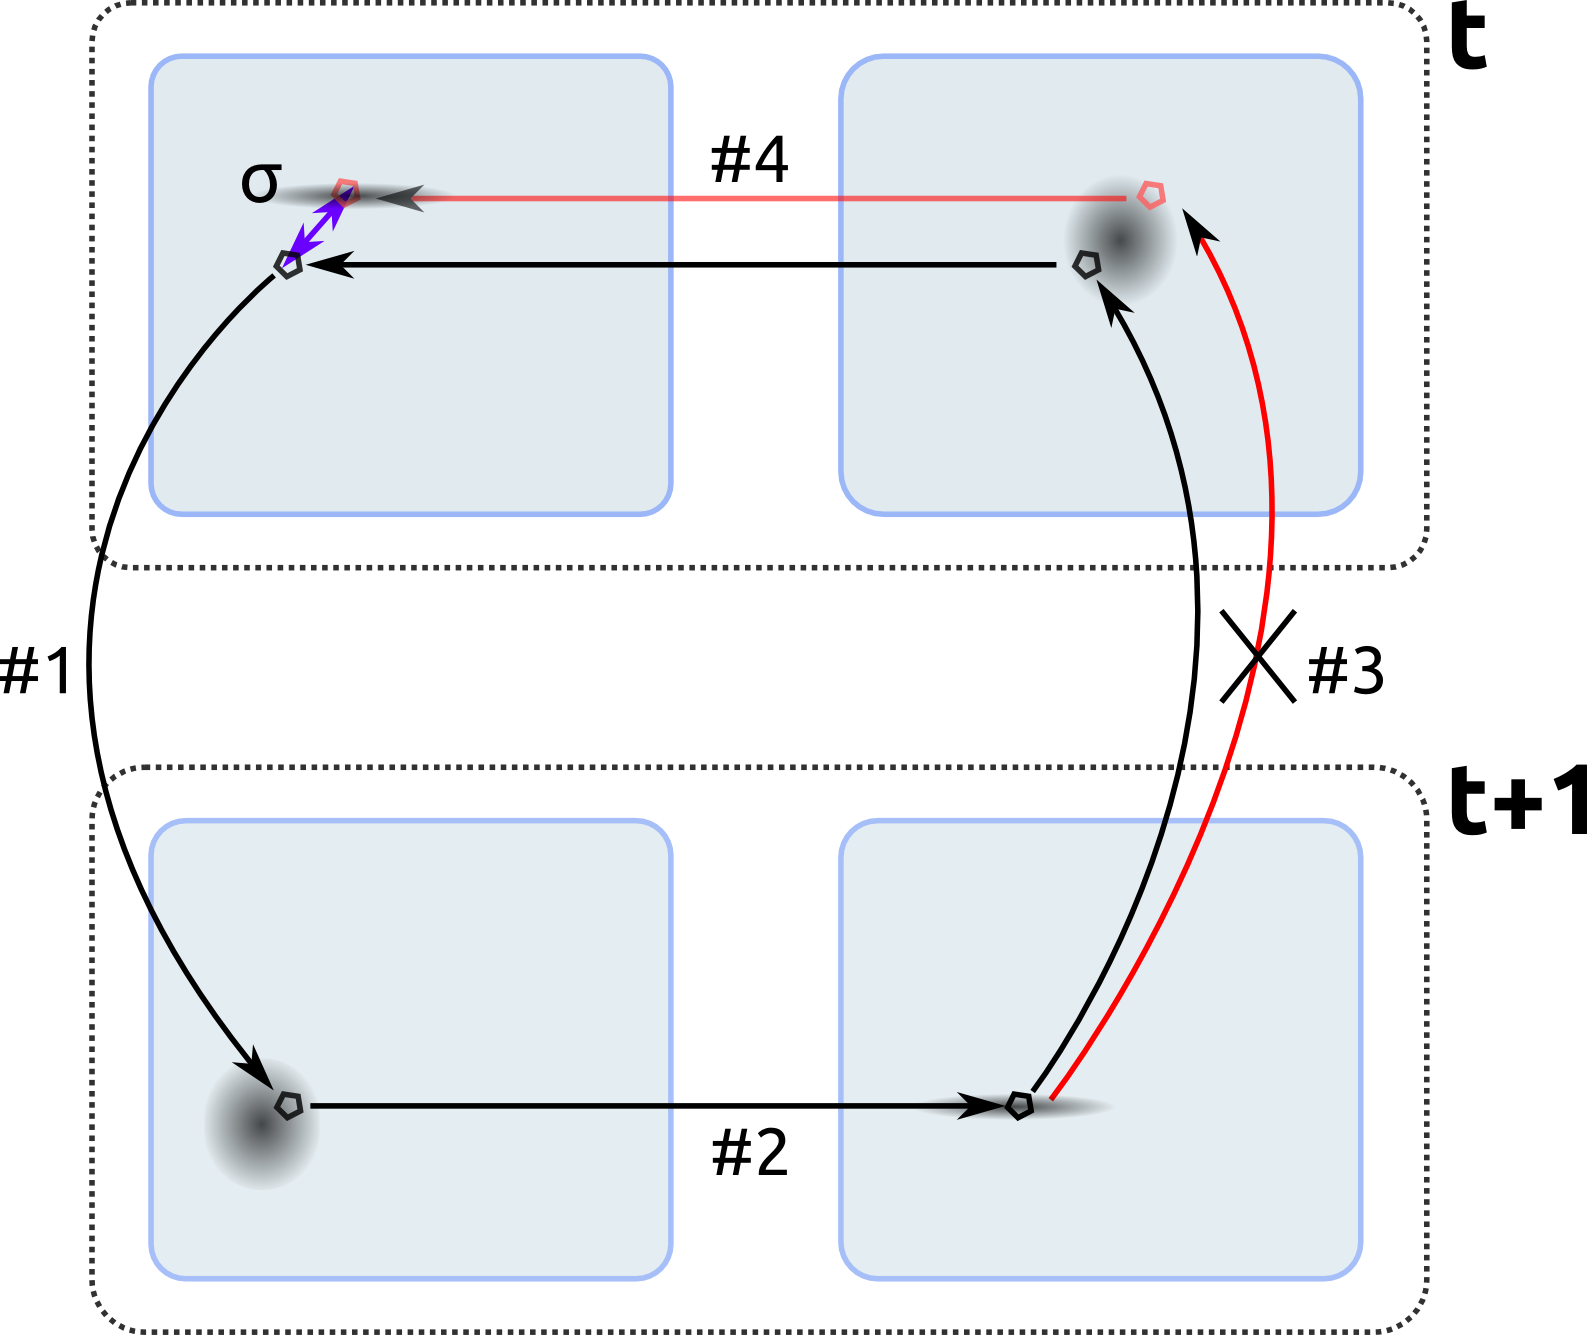
\includegraphics[width=0.5\textwidth]{Chapter3/graphics/4-Frames.png}
	\end{center}	
	\caption{Illustration du processus de suivi redondant de points, et de réjection de points fautifs. Un suivi fautif est illustré en rouge, tandis que les espaces de recherche des différents suivis sont marqués par une zone noircie.}
	\label{fig:ch3_4Frame}
\end{figure}

La Figure \ref{fig:ch3_4Frame}, nous permet par ailleurs d'illustrer les remarques suivantes. Les deux suivis de points dans le temps (étapes 1 et 3) ont un espace de recherche isotrope dans le plan image, tandis que les étapes 2 et 4 sont accélérées par une recherche sur les lignes uniquement. On comprend bien qu'un suivi de point parfait nous conduit à la position initiale, c'est-à-dire que la somme des déplacements calculés par les étapes 1,2,3 et 4 s'annulent. Dans cet exemple, le suivi de point de l'étape 3 est fautif, et nous conduit à l'écart $\sigma$ observé par comparaison entre la position de départ et celle d'arrivée.\\

\subsubsection{Détails de la méthode}
La position initiale des points à suivre est connue, car il s'agit des points correctement suivis à l'étape précédente, auxquels s'ajoutent les points d'intérêt nouvellement introduits. La procédure proposée pour la sélection de ces nouveaux points sera présentée par la suite (cf. \ref{sec:ch3_Sélection des points d'intérêt} et \ref{sec:ch3_Sélection dynamique des points d'intérêt}). On effectue ensuite quatre étapes de suivi de points, chaque étape utilisant la position obtenue lors du suivi précédent. Le critère de qualité final est individuel, il est lié pour chacun des points à la somme des déplacements obtenus lors de son suivi successif sur les 4 étapes proposées. Cette somme doit bien sûr être nulle dans le cas d'un suivi parfait, on fixe en pratique un seuil d'erreur maximal. Cette vérification est par ailleurs combinée au critère de perte de point intrinsèque à l'algorithme KLT (\ref{eq:ch3_KLT_iteration}) : si la matrice $G$ n'est pas inversible (si son déterminant est inférieur à un seuil $min_{det}$), le point est considéré comme perdu. Si l'on note ${d_{i,i+1}}^k$ le déplacement du point $k$ entre les images $i$ et $i+1$, $\sigma^k$ l'erreur mesurée lors de la procédure de suivi, et ${\delta_{i,i+1}}^k$ le statut obtenu après un suivi de point par l'algorithme KLT, on obtient la définition formelle de la validité $V^k$ de notre point :\\
\begin{align}
	\sigma^k 					=& \: \sum\limits_{i=0}^{3} {d_{i,j}}^k  \qquad (j = i+1 \: modulo \: 3)\\
	{\delta_{i,j}}^k :=& \: [ det(G_{i,j} > min_{determinant}] 	\\
	\delta_k 					=& \: \prod\limits_{i=0}^{3} \delta_{i,j}^k 				\\
	V^k 							=& \: [\sigma^k < {\sigma}_{max}] \times \delta_k
\end{align}

On pourra remarquer que la charge de calcul supplémentaire liée à cette procédure, si elle peut sembler considérable, n'est en réalité pas rédhibitoire. Le suivi de points entre les deux caméras est en effet simplifié par la rectification des images, qui permet de ne chercher les correspondances que sur un nombre de ligne limité, méthode souvent utilisée dans le calcul des cartes de disparité. Par ailleurs, l'algorithme KLT s'adapte très bien à cette procédure, dans le sens où les pyramides d'images et leurs gradients n'ont pas à être re-calculés dans le cadre de notre suivi redondant. La charge de calcul supplémentaire est ainsi uniquement liée aux itérations \ref{eq:ch3_KLT_iteration} et \ref{eq:ch3_KLT_pyramid}. Nous montrons dans \ref{sec:ch3_Implémentation} qu'il est possible de réaliser cette opération en temps réel et sur un grand nombre de points (plusieurs milliers) par une implémentation adaptée.

\subsection{Sélection de nouveaux points} \label{sec:ch3_Sélection des points d'intérêt}
\subsubsection{Principe}
La sélection de nouveaux points n'est pas aussi simple qu'un examen rapide pourrait le laisser supposer. L'utilisation d'un détecteur de points d'intérêt est évidemment requise, mais le critère de sélection des points est important. Le tri des points selon leur saillance conduirait ainsi à l'accumulation de points sur les zones les plus contrastées et texturées de l'image, tandis que d'autres zones peuvent rester inobservées. L'uniformité de la densité d'information est un critère important dans notre démarche (voir \ref{sec:ch3_densité informations}), tant on ne peut initialement préjuger des zones les plus porteuses d'informations. Par ailleurs, nous souhaitons pouvoir si besoin augmenter la densité de l'échantillonnage sur certaines zones préalablement identifiées, par exemple par un algorithme ou capteur tiers. \\

On propose finalement la procédure suivante, consécutive à la détection des points d'intérêts de l'image et à même de sélectionner les nouveaux points les plus appropriés :
\begin{itemize}
	\item \textbf{Rejet des points proches de l'existant:\\}
	Création d'un masque autour des points déjà présents, afin d'établir une distance minimale entre deux points suivis. \\
	
	\item \textbf{Sélection préférentielle dans les zones d'intérêt:\\} 
	Création d'un second masque lié aux zones dont on veut améliorer la connaissance. Il s'agit simplement d'évaluer la présence ou non des points testés dans les zones d'intérêt, le nombre de points choisis à l'intérieur et à l'extérieur de ces zones étant décrit par la suite.\\
\end{itemize}

Les nouveaux points sont systématiquement sélectionnés par le premier masque, puis l'utilisation du second masque est décrite dans \ref{sec:ch3_Sélection dynamique des points d'intérêt}. Le seuil de détection des points d'intérêt est volontairement fixé très bas dans notre implémentation, nous permettant de \og saturer\fg{} ce mécanisme de sélection. Ceci conduit cependant à des calculs inutiles, et un mécanisme de seuil adaptatif serait sans doute préférable.

\subsubsection{Intérêt de l'utilisation de masques}
En notant $N_{initiaux}$ le nombre de points présents initialement, et $N_{nouveaux}$ le nombre de points à introduire, avec $N_{initiaux} >> N_{nouveaux}$, l'intérêt d'une implémentation par masque peut se décrire en termes de complexité. L'ordre de grandeur des opérations à effectuer pour trier les points selon les critères précédents est en effet de $O(N_{initiaux} \cdot N_{nouveaux})$ pour une implémentation naïve par comparaison directe, contre $O(N_{nouveaux} + N_{initiaux})$ pour une implémentation par masque de réjection.\\

Il est à noter qu'une approche différente, à base d'arbres quaternaires (\emph{Quadtrees}), est également proposée par Mei et al. (\cite{Mei2010, Mei}) pour favoriser l'homogénéité des points sur l'image. Cette technique est couramment utilisée pour segmenter l'espace, une surface donnée pouvant être successivement subdivisée en 4 cellules indexées dans un arbre de décision, chaque feuille ayant dans ce cas 4 enfants, jusqu'à ce que la subdivision soit suffisamment petite. Dans leur approche, la répartition des points est explicitement uniforme à grande échelle, puis forcée à tous les étages de l'arbre tant que la détection de points d'intérêt dans la cellule désignée est concluante. \\
Cet algorithme se prête cependant mal à une distribution volontairement non-uniforme des points, comme nous le proposons ci-dessous, et nous avons supposé que ces deux approches étaient par ailleurs équivalentes en termes de rapidité d'exécution. On accepte cependant, avec notre implémentation, une perte d'uniformité qui nous conduit à favoriser les points d'intérêts de meilleure qualité.

\subsubsection{Mécanisme de sélection préférentielle des nouveaux points} \label{sec:ch3_Sélection dynamique des points d'intérêt}
Supposons ici que l'on veuille modifier dynamiquement la densité d'échantillonnage des points sur une image, en l'augmentant sur des zones distinctes d'un rapport $k$. On peut alors décrire un mécanisme permettant de tendre vers cette répartition grâce à une sélection adéquate de nouveaux points. On note pour ce faire $N_o^l$ le nombre de points à l'extérieur de la zone privilégiée lors de l'itération $l$, et $N_t^l$ le nombre de points à l'intérieur de cette zone visée lors de l'itération $l$. On note de même $S_o^l$ et $S_t^l$ les surfaces respectives des zones neutres et visées. On note enfin  $N_{o,i}^l$ (respectivement $N_{t,i}^l$) le nombre de points à introduire dans la zone neutre (respectivement visée) lors de l'itération $l$. On souhaite alors tendre vers $d_t = k \cdot d_o$ avec $d$ la densité d'information échantillonnée par unité de surface. 

\begin{align}
	d_t^{l+1} =& \: k \cdot d_o^{l+1} \\
	\frac{N_t^l + N_{t,i}^{l+1} }{S_t^{l+1}} =& \: k \cdot \frac{N_o^l + N_{o,i}^{l+1} }{S_o^{l+1}} \\
	N_{t,i}^{l+1} =& \: S_t^{l+1} \cdot k \cdot \frac{N_o^l + N_{o,i}^{l+1} }{S_o^{l+1}} - N_t^l 
\end{align}

Connaissant par ailleurs le nombre total de nouveaux points à introduire $N_i^{l+1} = N_{o,i}^{l+1} + N_{t,i}^{l+1}$ on obtient simplement :

\begin{align}
	N_{t,i}^{l+1} &= \:\frac{k \cdot \frac{S_t^{l+1}}{S_o^{l+1}} \cdot (N_o^l + N_i^{l+1}) - N_t^l}  {1 + k \cdot \frac{S_t^{l+1}}{S_o^{l+1}}} \\
	N_{o,i}^{l+1} = \: N_i^{l+1} - N_{t,i}^{l+1} &= \frac{ N_i^{l+1} + N_t^l - k \cdot \frac{S_t^{l+1}}{S_o^{l+1}} \cdot (N_o^l + N_i^{l+1})}  {1 + k \cdot \frac{S_t^{l+1}}{S_o^{l+1}}}
\end{align}

On a supposé dans le calcul précédent que nous disposions de suffisamment de points détectés pour satisfaire l'ensemble des contraintes ($N_{o,i}^{l+1}$ et $N_{t,i}^{l+1}$ sont saturables, c'est-à-dire que l'on a détecté suffisamment de points pour les ajouts effectifs soient ceux prévus par l'algorithme). Dans le cas contraire, on fait le choix de ne pas respecter la répartition demandée afin de privilégier le renouvellement des points perdus par rapport à leur répartition dans l'image. On ne propose donc pas un algorithme déterministe, mais une \og pression de sélection\fg{} quant à l'ajout de nouveaux points qui doit nous permettre de tendre vers une répartition souhaitée. \\

Dans le cas où les points détectés seraient trop nombreux (relativement à un seuil arbitraire, fixé à 5000 points dans notre implémentation), on exploite tout d'abord un mécanisme dit de "<sélection par tas\fg{} (\emph{heap select}), similaire au "<tri par tas\fg{} sans produire toutefois de sélection triée. Le critère de qualité utilisé pour la sélection est la réponse au détecteur de points d'intérêt, qui varie selon les méthodes (cf. section \ref{sec:ch3_Détection_points_intérêt}).\\

Un exemple de résultat est visible sur la Figure \ref{fig:ch3_Weighted_selection}, dans laquelle le rapport de densité demandé entre l'intérieur et l'extérieur de la ROI (\emph{Region Of Interest }, zone d'intérêt) est inférieur à 1. On souhaite donc éviter d'échantillonner cette zone, ce qui pourrait par exemple correspondre au suivi d'un véhicule dont la position est connue. On constate bien que la densité des points est très inférieure à l'intérieur de la zone d'exclusion, comme souhaité. \\

La complexité de ce mécanisme de sélection n'est que marginalement augmentée par rapport à l'usage d'un masque simple qui évite l'accumulation, et reste de l'ordre de $O(N_{nouveaux} + N_{initiaux})$.

\begin{figure}[h]
	\begin{center}
		\begin{subfigure}{0.58\textwidth}
		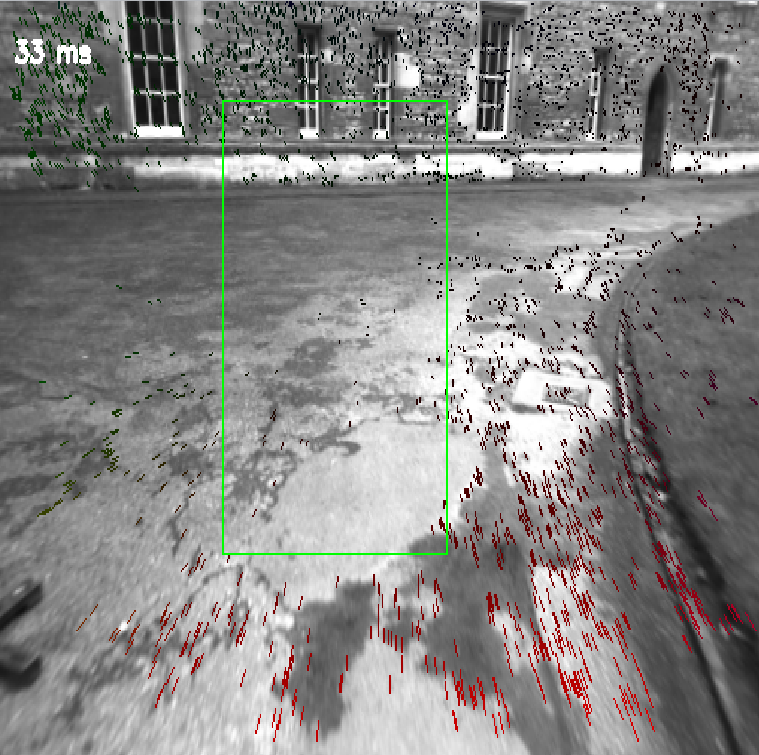
\includegraphics[width=\textwidth]{Chapter3/graphics/Detectors_weighted.png}
		\caption{La zone délimitée en vert correspond à une densité souhaitée plus faible.}
		\end{subfigure}	
		~
		\begin{subfigure}{0.38\textwidth}
			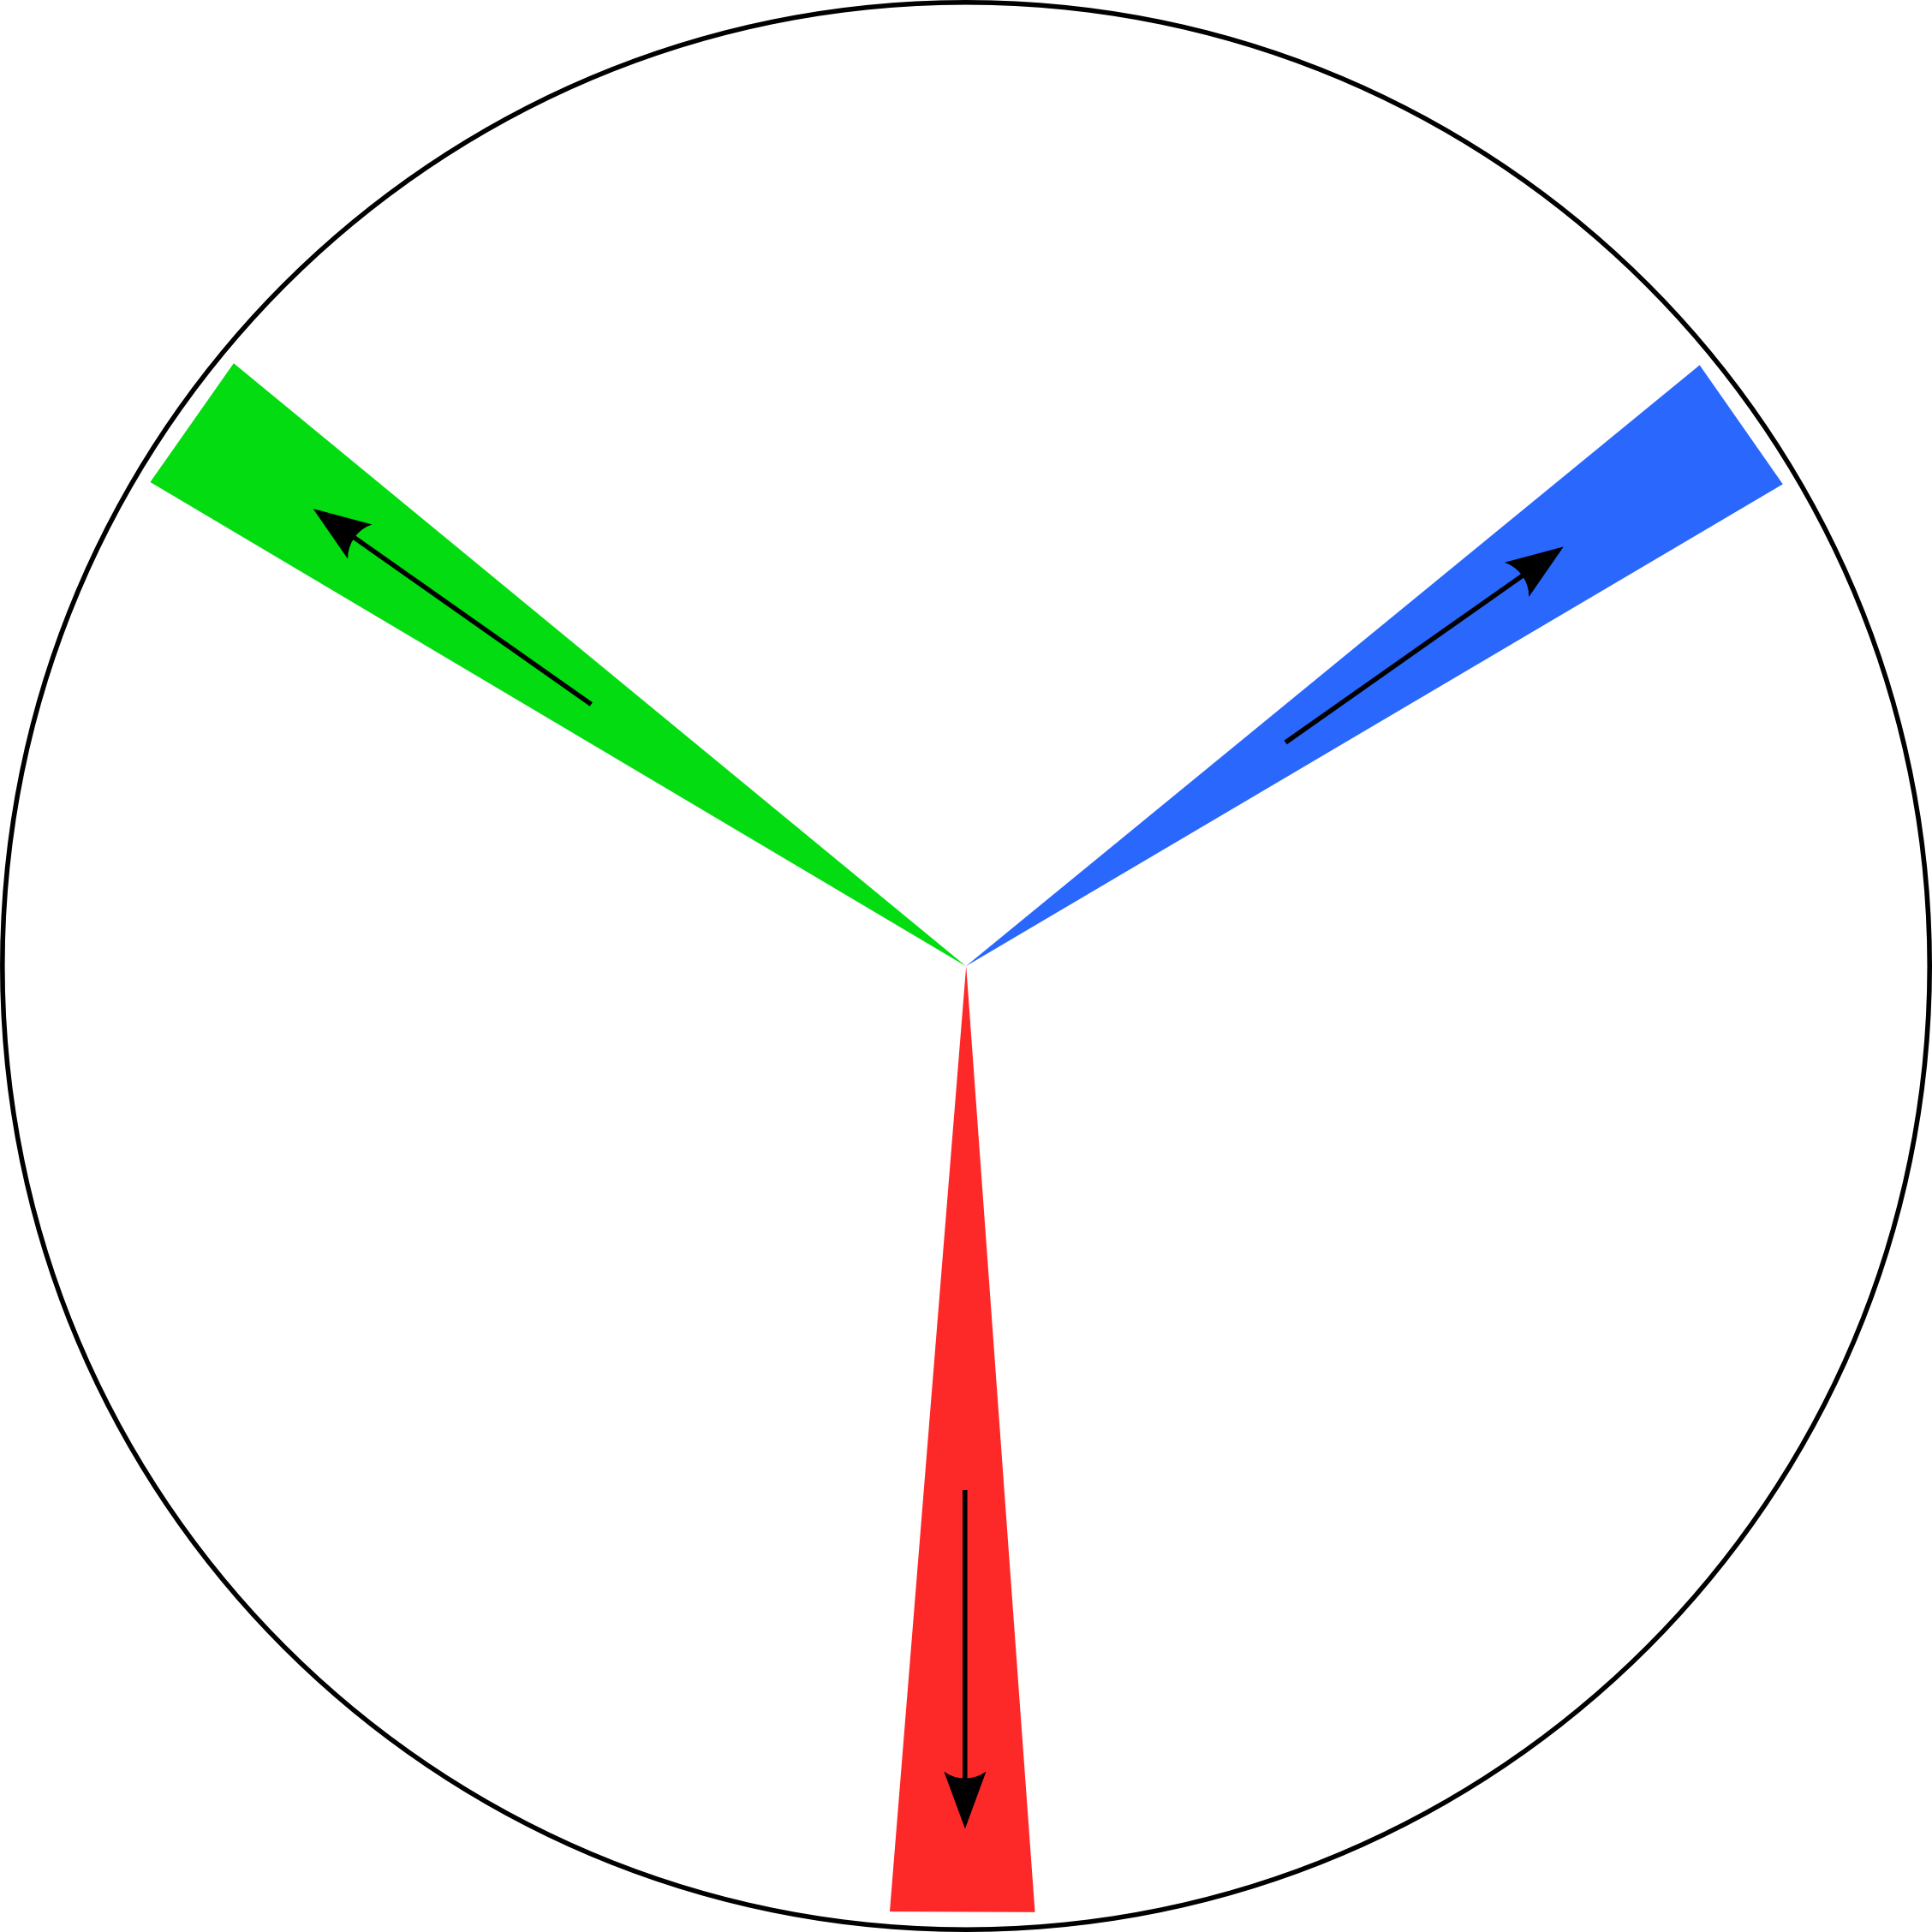
\includegraphics[width=\textwidth]{Chapter3/graphics/directions_chroma.png} 
			\caption{Code couleur représentant les directions des vecteurs de déplacement dans le plan image}
			\label{fig:ch3_code_couleur}
		\end{subfigure}	
	\end{center}
	\caption{Exemple de résultat de l'algorithme de sélection préférentielle des nouveaux points d'intérêt}	
	\label{fig:ch3_Weighted_selection}
\end{figure}

\section{Implémentation et évaluation}
\subsection{Détection de points d'intérêt}\label{sec:ch3_Eval_PI}
Comme abordé dans \ref{sec:ch3_Détection_points_intérêt}, de nombreux détecteurs de points d'intérêt sont présents dans la littérature, et la recherche d'un algorithme les surpassant n'était pas l'objet de cette thèse. Nous avons cependant comparé quelques uns des détecteurs les plus utilisés dans la littérature, par rapport à nos besoins. Trois critères nous semblent en effet importants dans notre perspective d'un traitement temps réel sur de nombreux points suivis dans le temps : 
\begin{itemize}
	\item le nombre de points détectés doit être important pour justifier notre démarche, supérieur à 4000 points en pratique,.
	\item le temps de détection doit être le plus faible possible, cette opération étant renouvelée à chaque itération,
	\item la qualité des points sélectionnés doit être la plus grande possible, dans le sens ou le suivi de points redondant mis en place (\ref{sec:ch3_Suivi redondant}) doit permettre de conserver le plus de points possibles d'une itération sur l'autre tout en conservant une couverture la plus homogène possible.
\end{itemize}

Le premier point ici soulevé n'est pas discriminant : chacun des détecteurs envisagés est associé à un seuil de détection, et l'ajustement de celui-ci autorise en pratique, dans tous les cas, suffisamment de nouveaux points. On évalue donc dans ce qui suit les deux points suivants. La séquence utilisée est tirée de la banque de données \textit{New College} (\cite{Smith2009}), acquise par des caméras stéréoscopiques \textit{Point Grey Lady Bug 2}. Ces images ont une taille de 512 x 384 pixels, en niveaux de gris, sur une profondeur de 8 bits.

\subsubsection{Comparaison: temps de calcul}
On compare dans le tableau \ref{tab:ch4_temps_de_calcul} le temps de calcul lié à l'usage des détecteurs Harris, SIFT, SURF, \og Shi et Tomasi\fg{} et FAST sur une séquence d'images. Leurs seuils respectifs autorisent une détection de plus de 4000 points par image. On compare à la fois le temps lié à la détection de points d'intérêt et le temps lié au suivi de points, pour éventuellement prendre en compte un problème lié à une détection de points moins efficace mais plus rapide dans l'absolue dans le cadre de l'algorithme KLT. Le suivi des points est ici confié à une implémentation pyramidale de l'algorithme KLT, exécutée sur le CPU. Les temps de calcul correspondent à une implémentation en C++ exploitant la libraire OpenCV, sur un processeur Core i7 2GHz. On vérifie la constance du temps de détection et de suivi de points sur 300 images, les variations relatives de temps de calcul étant faibles on ne présente ici que les temps moyens. \\

\begin{table}[H]	
	\begin{center}
			\begin{tabular}{| c | c | c | c |} 
				\hline
				Détecteur 					& \pbox[c]{3cm}{\centering {Temps de \newline détection (ms)}} & \pbox[c]{3cm}{\centering {Temps du suivi \newline (ms)}} & \pbox[c]{3cm}{\centering {Temps total \newline (ms)}}\\
				\hline
				\textnormal{FAST}						& 6 	&	54	& 60 	\\
				\hline
				\textnormal{Harris} 				& 10 	&	50	& 60 	\\
				\hline
				\textnormal{Shi \& Tomasi} 	& 11 	&	50	& 61 	\\	
				\hline
				\textnormal{SURF} 					& 33 	&	59	& 91 	\\	
				\hline
				\textnormal{SIFT} 					& 74 	&	54	& 128	\\ 
				\hline
			\end{tabular} 
	\end{center}
	\caption{Comparaison des temps de calcul liés à différentes méthodes de détection, pour 4000 points suivis.}
	\label{tab:ch4_temps_de_calcul}
\end{table}

On constate aisément sur le tableau \ref{tab:ch4_temps_de_calcul} que le temps de calcul lié à l'utilisation des détecteurs SURF et SIFT est rédhibitoire. On n'extrait pas pour ces derniers de descripteur associé, ce qui est par ailleurs une caractéristique recherchée de ces algorithme. Le détecteur FAST est le plus rapide avec une moyenne de 6 ms par frame, suivi par les détecteurs Harris et \og Shi et Tomasi\fg{}. L'intégration de l'étape de suivi de points permet de ramener ces trois derniers algorithmes à une quasi-équivalence. L'algorithme KLT n'offre en effet pas un temps de calcul constant, les critères d'arrêt (outre le nombre maximal d'itérations) étant la stabilisation de la convergence et une matrice G non-inversible.

\subsubsection{Comparaison: qualité}
\paragraph{Perte des points lors du suivi\\}
On compare maintenant la qualité des détections, dans le cadre de nos besoins particuliers. On commence par mesurer pour cela le nombre de points perdus par itération, selon notre critère de cohérence présenté dans \ref{sec:ch3_Suivi redondant}. La tolérance est ici fixée à $\sigma_{max}$ = 1,5 pixel. On peut remarquer que des points sont nécessairement perdus dans cette procédure, la caméra se déplaçant pendant la séquence et modifiant donc son champ de vision. Le nombre total de point suivi dans ce test est de 4000 points.

\begin{figure}[h]
	\centerline{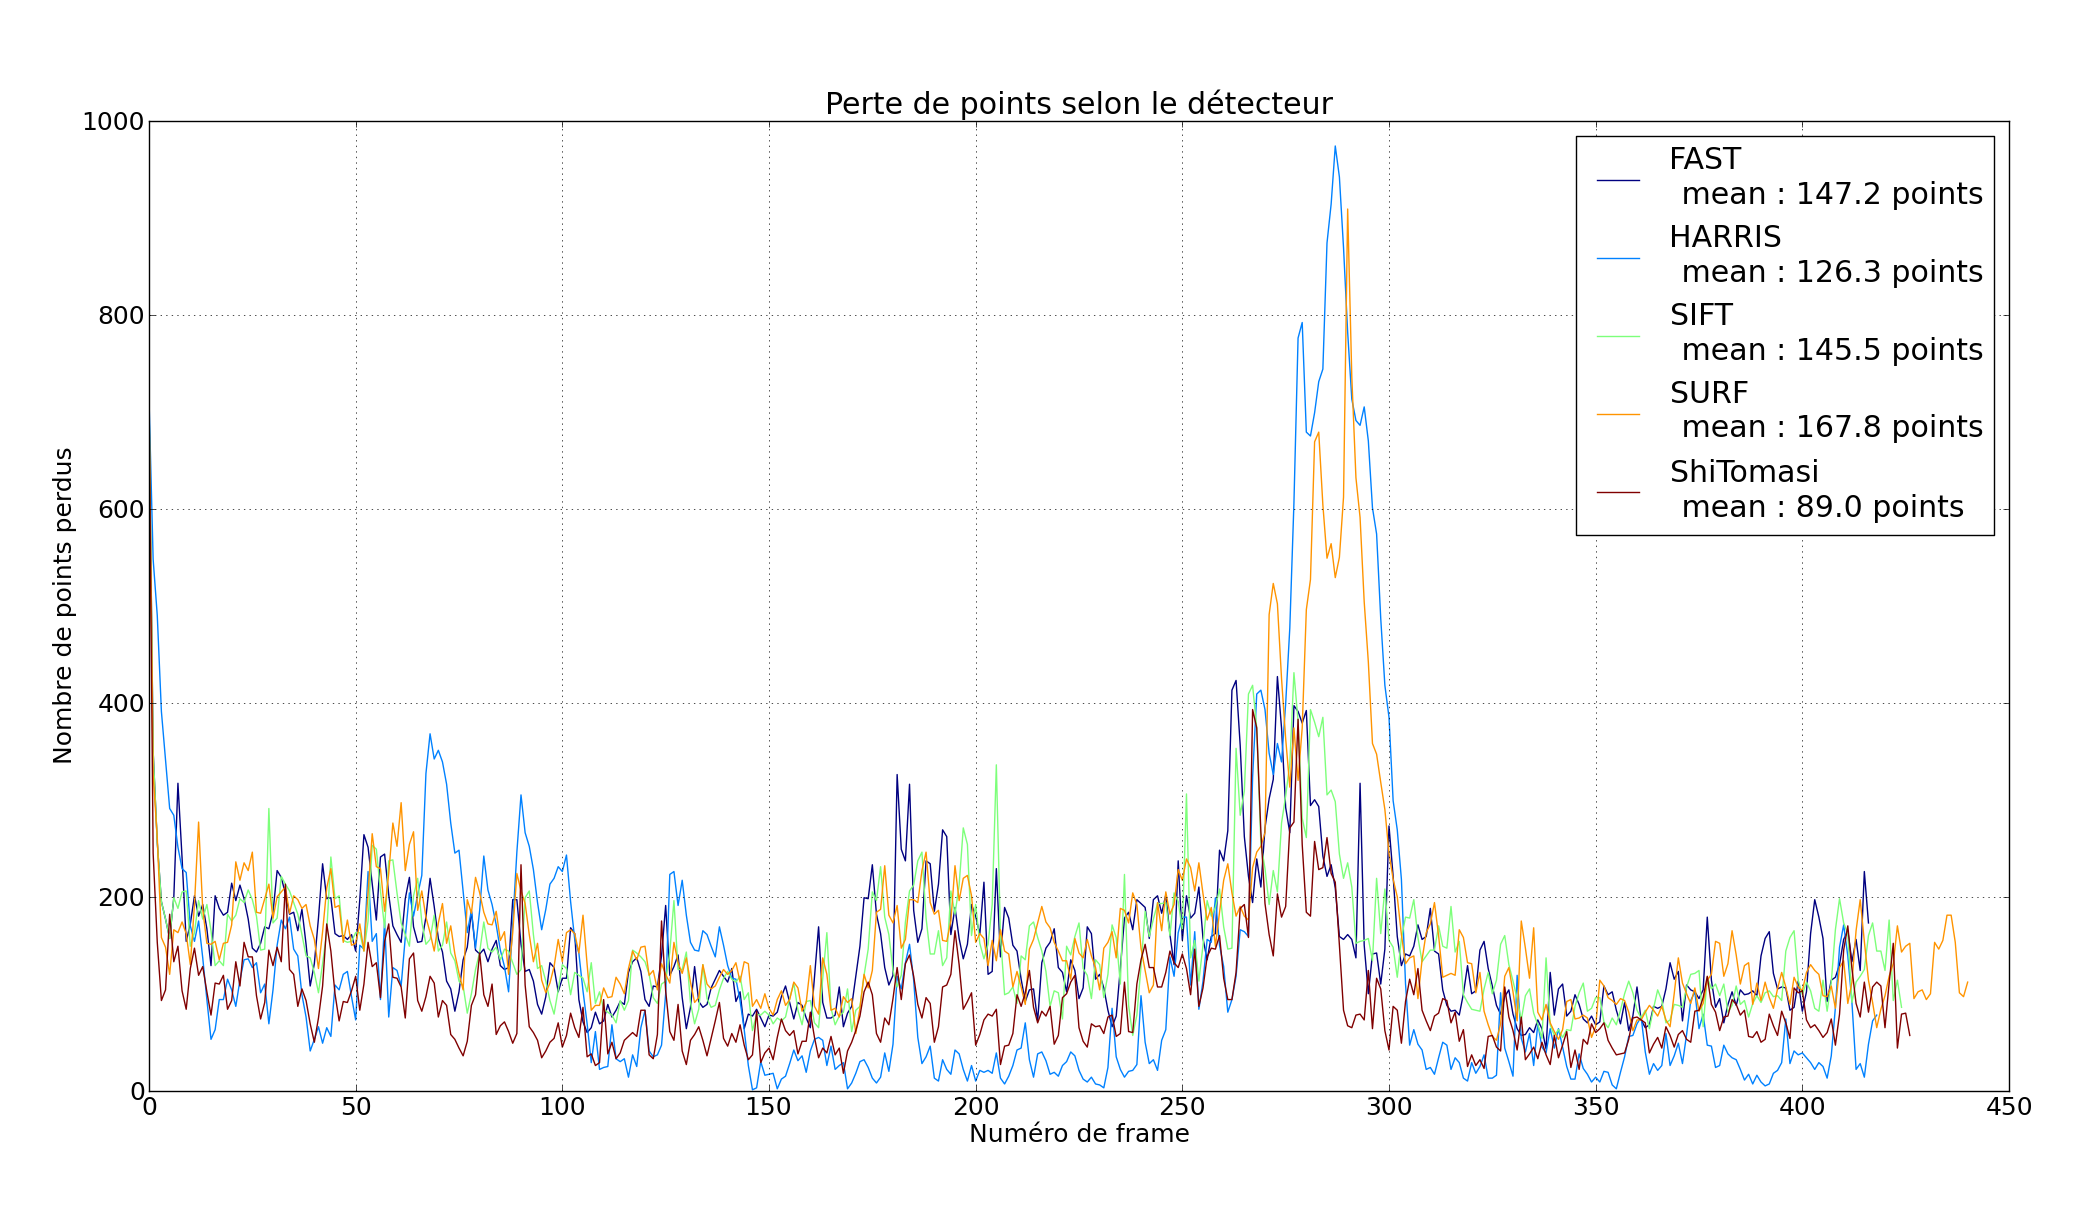
\includegraphics[width=\textwidth]{Chapter3/graphics/Detectors_comparison_q_clean.png}}
	\caption{Comparaison de la qualité des points suivis : évolution du nombre de points perdus pour 5 détecteurs : FAST, Harris, SIFT, SURF et Shi et Tomasi. Les meilleures performances sont obtenues par Shi et Tomasi.}
	\label{fig:ch3_Vision_robustesse}
\end{figure}

La Figure \ref{fig:ch3_Vision_robustesse} nous montre que tous les détecteurs ne fournissent pas des points aussi robustes dans le cadre de notre procédure de suivi par KLT. Les points obtenus par Shi et Tomasi ainsi que les points de Harris occasionnent le moins d'erreur de suivi. On peut par ailleurs constater que le nombre de points perdus peut évoluer de manière significative au cours du temps, du fait des mouvements de la caméra, ce qui met l'accent sur un processus de redistribution des points efficace.

\paragraph{Uniformité\\} \label{Vision_uniformité}
Le nombre de points perdus par itération ne rend cependant pas compte de l'ensemble de nos besoins, l'uniformité de la couverture étant par ailleurs un aspect important. Cette couverture de la scène par les points échantillonnés ne dépend pas seulement de la détection initiale, mais également de la qualité des points détectés, dans la mesure où le suivi des points dans le temps peut modifier cette répartition. On peut constater en comparant la répartition de la population de points suivis (Figure \ref{fig:ch3_Vision_uniformité}), suite à l'usage de deux détecteurs spécifiques pendant un grand nombre d'itérations, que celle-ci diffère grandement quand bien même le reste de l'algorithme est conservé (notamment le rejet par masque des nouveaux points trop proches des points existant, cf. section \ref{sec:ch3_Vision_mécanisme}).

\begin{figure}[h]
	\begin{center}
		\begin{subfigure}{0.48\textwidth}
			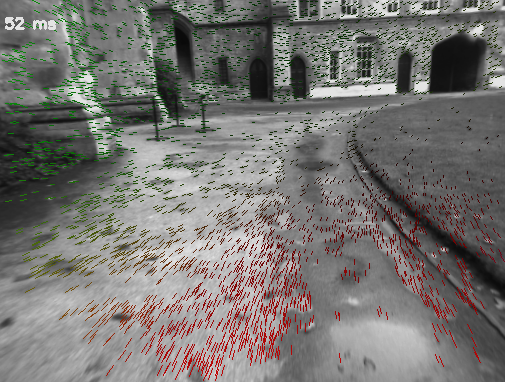
\includegraphics[width=\textwidth]{Chapter3/graphics/Detectors_FAST_init.png} 
			\caption{Détecteur FAST - première détection}
		\end{subfigure}	
		~	
		\begin{subfigure}{0.48\textwidth}
			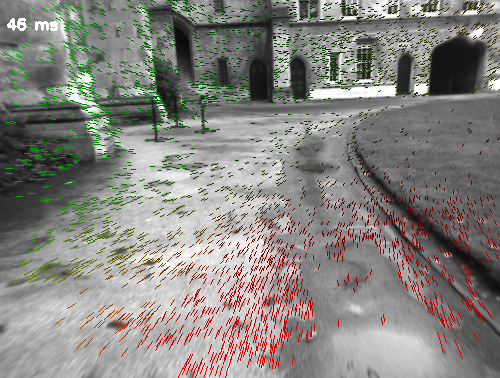
\includegraphics[width=\textwidth]{Chapter3/graphics/Detectors_HARRIS_init.png} 
			\caption{Détecteur Harris - première détection}
		\end{subfigure}
		\\
		\begin{subfigure}{0.48\textwidth}
			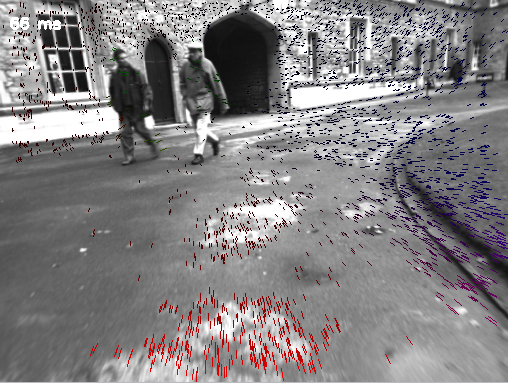
\includegraphics[width=\textwidth]{Chapter3/graphics/Detectors_FAST.png} 
			\caption{Détecteur FAST - 300 itérations}
		\end{subfigure}
		~
		\begin{subfigure}{0.48\textwidth}
			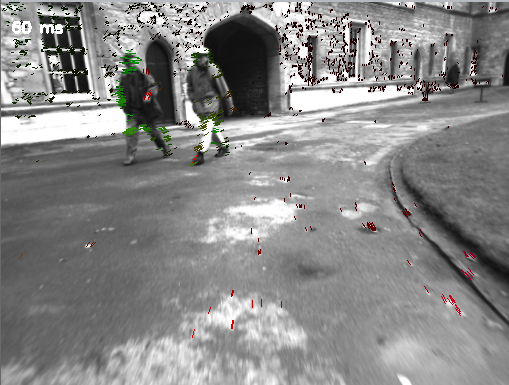
\includegraphics[width=\textwidth]{Chapter3/graphics/Detectors_HARRIS.png}
			 \caption{Détecteur Harris - 300 itérations}
		\end{subfigure}
		
		\caption{Comparaison de la qualité des points suivis : répartition des points après 300 itérations.}	
		\label{fig:ch3_Vision_uniformité}
	\end{center}
\end{figure}

L'explication de cette différence entre ces deux détecteurs est liée aux caractéristiques des points d'intérêt retenus (qui diffèrent grandement selon les détecteurs, comme nous l'avons vu dans \ref{sec:ch3_Détection_points_intérêt}), et à la tolérance accordée au suivi redondant des points (\ref{sec:ch3_Suivi redondant}). Les points détectés peuvent ainsi dériver au fil des itérations du fait de l'imperfection de l'étape de suivi dans le temps, et éventuellement converger vers les mêmes localisations, ce qui contrarie notre ambition d'une couverture angulaire maximale et uniforme. Ce phénomène est patent sur les images de la Figure \ref{fig:ch3_Vision_uniformité}, dans laquelle (dans le cas de l'utilisation de Harris) les points ont \og glissé\fg{} le long des arrêtes. On propose donc de quantifier l'uniformité de la répartition des points par l'étude du nombre de points par unité de surface, sur un pas suffisamment faible pour mettre en valeur les discontinuité de densité. \\
On représente sur la figure \ref{fig:ch3_Vision_densité} la fonction de répartition des points sur l'image en fonction de leur densité locale, avec le procédé suivant : chacun des éléments de surface de l'image (que l'on choisit suffisamment petit) peut recevoir un ou plusieurs points d'intérêt. On représente sur l'axe des abscisses la densité (croissante) de ces éléments de surface, tandis que l'axe des ordonnées représente le nombre de points présents dans des éléments de surface recevant cette densité de points. L'unité élémentaire de surface est choisie par rapport au nombre de points dans l'image, de sorte que théoriquement \textit{chaque unité de surface doit recevoir un unique point d'intérêt en cas de répartition uniforme}. Une distribution plus uniforme est donc plus présente sur la gauche du graphique. Autrement dit, l'axe des abscisses représente le degré de non-uniformité de la fonction de répartition. Cette étude est réalisée après 300 itérations, pour se placer en régime stabilisé, on utilise là encore les données de New College (\cite{Smith2009}).

\begin{figure}[H]
	\centering
	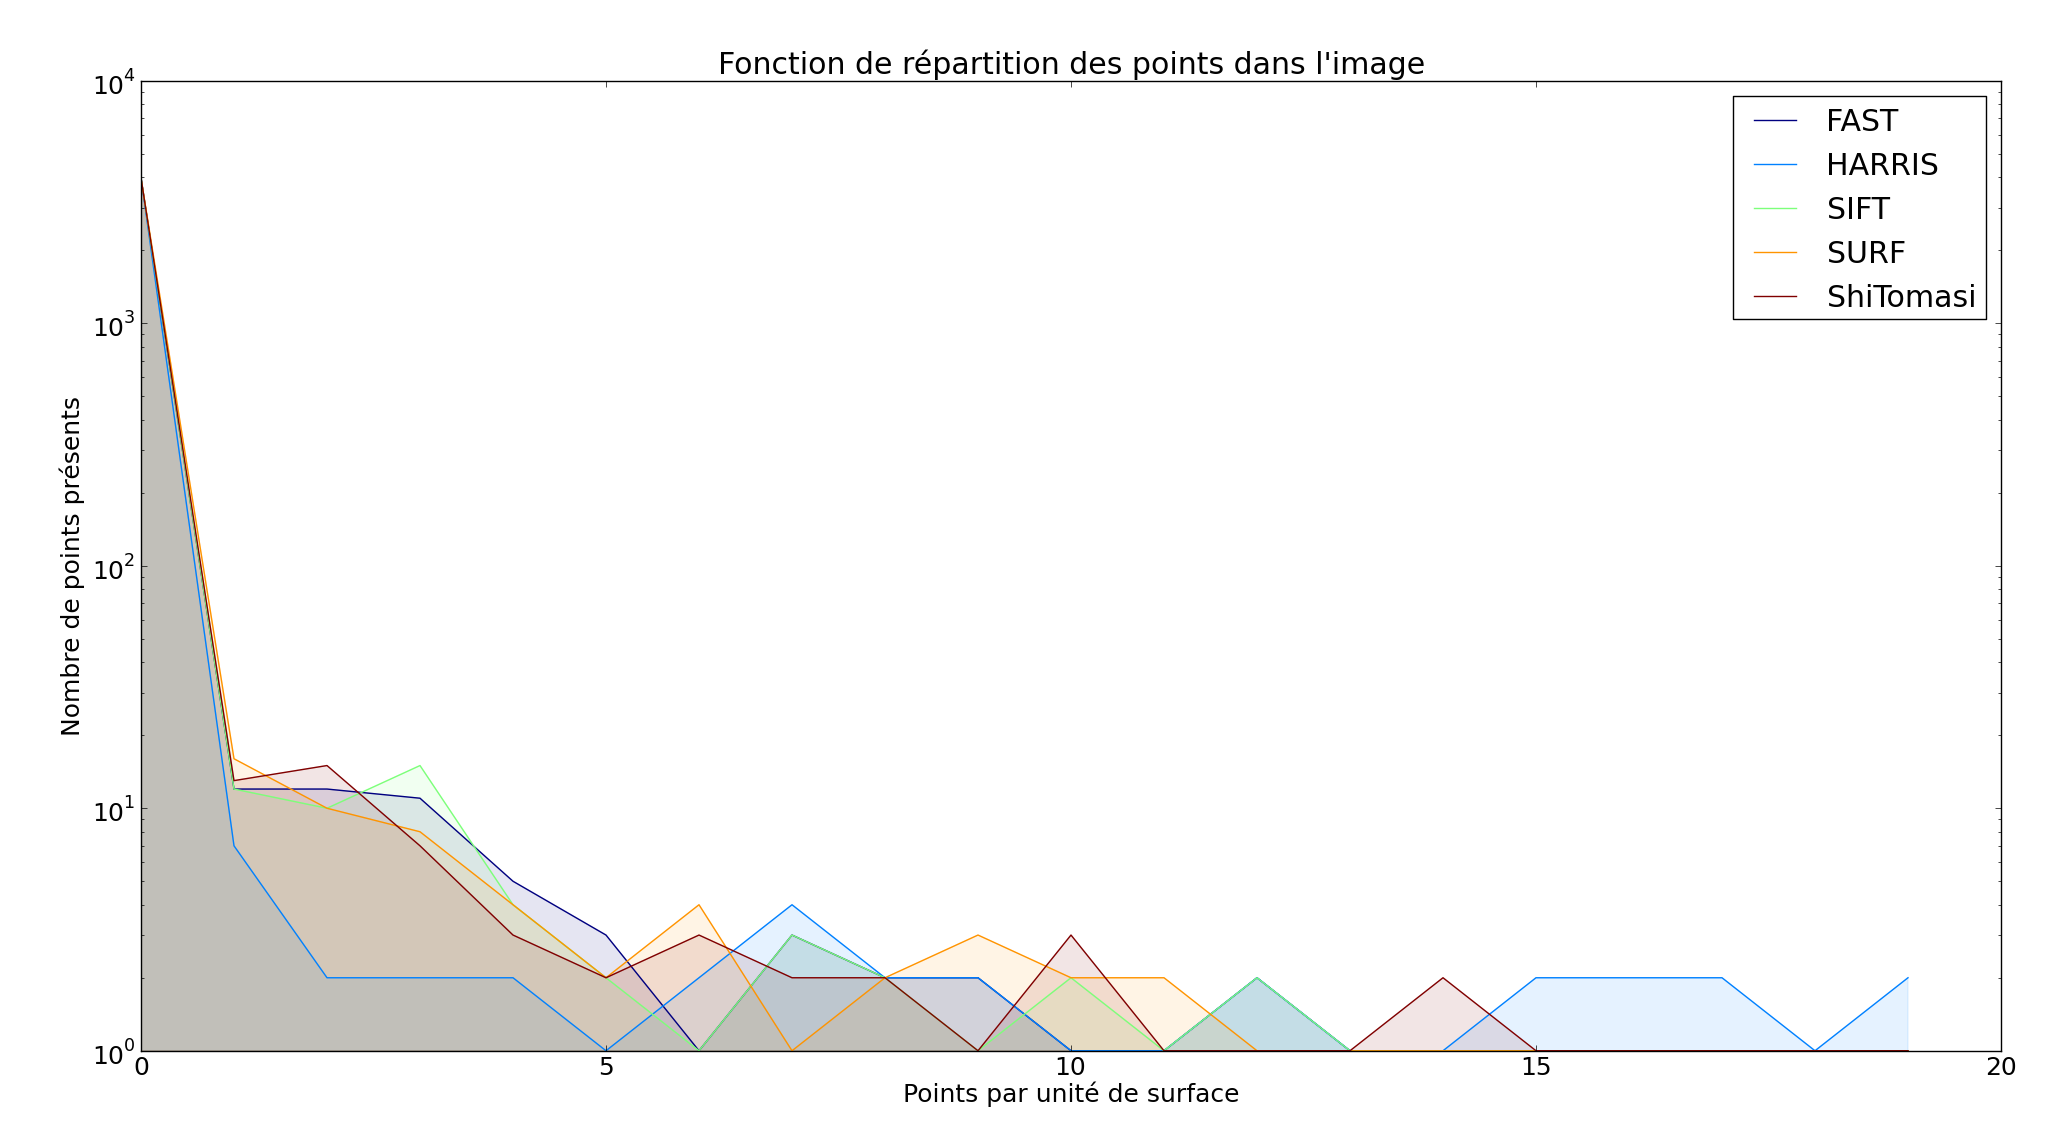
\includegraphics[width=\textwidth]{Chapter3/graphics/Detectors_comparison_density.png}
	\caption{Répartition des points après 300 itérations : mesure de l'uniformité du nombre de points par unité de surface}
	\label{fig:ch3_Vision_densité}
\end{figure}

On constate sur la figure \ref{fig:ch3_Vision_densité} que les points de Harris conduisent effectivement à une répartition moins uniforme. Les points SIFT et SURF sont par ailleurs marginalement meilleurs que les points FAST et Shi et Tomasi, ce qui tend à montrer que les points sélectionnés par ces détecteurs dérivent moins. Cette étude ne vaut bien sûr que pour des points suivis dans le temps par la méthode proposée par Lucas et Kanade, les conclusions pourraient être différentes avec une autre méthode de suivi. \\

\paragraph{Choix du détecteur:\\}
Au vu des évaluations réalisées pour ces différents détecteurs, il nous apparaît que les détecteurs SIFT et SURF, bien que de qualité, sont trop coûteux pour une implémentation visant un traitement temps réel. Les points de Harris, bien que rapides à détecter, se révèlent difficiles à suivre sur une séquence d'images, et contredisent notre effort initial visant à une couverture la plus complète possible du champ de vision. Les points FAST et ceux proposés par Shi et Tomasi nous semblent tous deux convenir au vu de ces évaluations, les second étant cependant plus adaptés au suivi de points par KLT. Il s'agit par conséquent des points que nous avons retenu pour la suite de notre implémentation.

\subsection{Suivi de points} \label{sec:ch3_Implémentation}
Le mécanisme proposé dans ce manuscrit pour le suivi de points, s'il n'est pas nouveau (il est notamment utilisé dans \cite{Lategahn2011} pour le suivi des points utilisés dans la détermination de l'ego-motion, ou dans \cite{Lenz2011}), n'a à notre connaissance jamais été mis en œuvre pour le suivi de l'intégralité des points d'intérêt considérés, sans doute du fait des contraintes associées au temps de calcul.\\
On peut dissocier schématiquement, du point de vue du suivi de points dans une approche de stéréo-vision, l'acquisition d'informations temporelles et spatiales selon que l'on considère les paires intra ou inter-caméras du schéma \ref{sec:ch3_Suivi redondant}. Lategahn propose ainsi un sous échantillonnage des mesures dans le temps (dans le sens où peu de points sont suivis dans le temps) pour mieux densifier la perception de l'environnement (la carte de disparité est calculée de manière dense). Cette méthode autorise la reconstruction d'un environnement très dense, mais se prive par la même de la perception d'un environnement mobile. Les méthodes présentes dans la littérature comportent le plus souvent ce compromis : seuls quelques points sont suivis sur l'ensemble du parcours redondant possible, tandis qu'un suivi dense est réalisé entre les caméras (carte de profondeur dense, par exemple \cite{Agrawal2007}) ou dans le temps (flux optique dense, par exemple \cite{Dumortier}).\\
La perception des objets en mouvement étant l'une de nos priorités, nous avons fait le choix de suivre autant de points dans le temps qu'entre les deux caméras, afin que le nuage de points obtenu puisse être indifféremment composé de points mobiles. Ceci peut poser des problèmes de performances, le temps de traitement d'une telle méthode étant potentiellement incompatible avec une exécution en temps réel. Nous avons donc évalué plusieurs approches pour tenter d'y remédier, et présentons ci-dessous quelques uns des résultats obtenus.

\subsubsection{Implémentation OpenCV}
Le mécanisme décrit dans \ref{sec:ch3_Suivi redondant} est assez simplement réalisable en utilisant les algorithmes disponibles dans la librairie OpenCV. Une implémentation naïve, utilisant notamment le logiciel RTMaps pour la synchronisation multi-capteurs, a été initialement réalisée afin de vérifier la faisabilité et la pertinence de cette approche. Le temps de calcul observé pour une implémentation native (C++) et pour le suivi de 4000 points est de l'ordre de 40 ms par itération pour une fenêtre de recherche de KLT de 6x6 pixels (sur une plate-forme Intel Core i7 à 2GHz), soit un traitement possible d'environ 25 images par seconde. \\
On souhaite traiter le plus grand nombre de point possible, afin de s'approcher des techniques denses, et de minimiser le risque d'un obstacle non perçu par sous-échantillonnage. Comme nous le verrons par la suite, cette partie visuelle est le facteur limitant de notre proposition, en termes de temps de traitement pour un grand nombre de points suivis (cf. \ref{sec:ch6_temps_reel}). Il était donc intéressant d'évaluer une implémentation plus rapide. L'utilisation de notre méthode sur des supports dont la puissance de calcul est limitée était enfin une seconde motivation pour aller au-delà d'une implémentation naïve.

\subsubsection{Pourquoi paralléliser ?}
\paragraph{Considérations générales:\\}
Une règle décrivant les gains consécutifs à une exécution parallèle a été proposée par Gene Amdahl dans les années 1960 (\cite{Amdahl1967}), qui montre simplement que celui-ci sera limité par la partie séquentielle du programme. Cette règle s'obtient en dérivant le calcul du temps d'exécution de manière assez simple, mais sa forme condensée est très intéressante. Si l'on note $P$ la proportion de la partie parallélisable du problème, et $S$ l'accélération qui peut être appliqué sur cette partie (par exemple le nombre d'unités d'exécution), la loi d'Amdahl s'écrit :

\begin{equation} \label{eq:ch3_Amdahl}
	gain = \frac{1}{1 - P + \frac{P}{S}}
\end{equation}

Autrement dit, si 70\% du programme est parallélisable, et que l'on peut le répartir sur 8 unités d'exécution concurrentes (P = 0.7, S = 8), le gain de vitesse (défini par le ratio des temps de calcul) attendu par une implémentation parfaite sera de 2.6, bien loin du rapport 8 que l'on aurait pu naïvement supposer.\\

\paragraph{Application à notre cas:\\}
Si l'on reprend l'algorithme de Lucas et Kanade (\ref{sec:ch3_KLT}) sous sa forme pyramidale (Bouguet, \cite{Bouguet2001a}), on peut le schématiser par quelques étapes :
\begin{enumerate}
	\item Construction des pyramides d'images (mise à l'échelle).
	\item Calcul de la carte du gradient sur la pyramide d'images. 
	\item Itérations de \og descente de gradient\fg{} pour tous les étages de la pyramide, pour retrouver sur l'image B la position d'un point de l'image A.\\
\end{enumerate}

Les deux premières opérations sont indépendantes du nombre de points suivis, contrairement à la troisième. Ces trois étapes sont interdépendantes, on ne peut donc pas imaginer de parallélisation macroscopique (exécuter ces trois étapes en même temps). Il est difficile d'estimer exactement la proportion $P$ du programme qui est parallélisable, au vu de ces trois étapes grossières. On peut cependant faire quelques observations :

\begin{itemize}
	\item La troisième étape est trivialement parallélisable, s'agissant d'optimisations indépendantes pour chaque point recherché.
	\item Les deux premières étapes sont éventuellement parallélisables, en morcelant l'image par exemple, mais des conditions aux limites s'appliquent (la parallélisation ne peut atteindre 100\%).
	\item La troisième étape devient prédominante en termes de temps de calcul quand le nombre de points à traiter augmente.\\
\end{itemize}

Si nous considérons la loi d'Amdahl, la structure générale de l'algorithme KLT, le fait que ce suivi de points soit le facteur limitant de notre algorithme global en termes de temps de calcul, et enfin notre prérequis du suivi d'un grand nombre de points au cours du temps, la parallélisation de KLT devient un élément important pour nous et justifie un travail complémentaire.\\
Les versions les plus récentes d'OpenCV intègrent une exécution parallélisée de cet algorithme de suivi de points sur le CPU, le temps de calcul de 40 ms annoncé précédemment intégrant cette amélioration. Compte tenu des possibilités d'exécution d'algorithmes sur des circuits hautement parallélisés, popularisés ces dernières années par les interfaces de programmation CUDA et OpenCL, nous avons donc considéré une implémentation spécifique de KLT profitant de leurs avantages.

\subsubsection{Implémentation GPU}
Le circuit dit GPU (\emph{Graphics Processing Unit}, Unité de calcul des graphismes), par opposition au CPU (\emph{Central Processing Unit}, Unité centrale de calcul) est historiquement présent sur les plates-formes de calcul grand public depuis l'avènement des rendus d'environnement en trois dimensions et en temps réel, souvent associés au jeux vidéos. Il s'agit d'un circuit initialement dédié au traitement des instructions de rendu, qui offrent un grand degré de parallélisme, et son architecture est donc adaptée à la gestion simultanée d'un grand nombre de processus. Son exploitation dans un cadre plus généraliste de calcul partagé (on parle alors de GPGPU - \emph{General Purpose Graphics Processing Unit}, Unité de calcul générique) est mise en avant depuis plusieurs années par quelques uns de ses concepteurs, qui y ont vu un relais de croissance et une exploitation aisée d'un savoir-faire déjà présent dans un nouveau domaine. Les interfaces de programmation CUDA, et plus récemment OpenCL, proposent ainsi d'intégrer à un programme classique (par exemple en C++) une partie déportée sur ces unités de calcul massivement parallèles, au prix d'une adaptation des algorithmes aux spécificités de ces architectures. \\

Notre approche se focalisant sur une grande densité d'échantillonnage dans une problématique de détection d'obstacles, et étant limitée par le temps de traitement de l'acquisition d'indices visuels, nous avons supposé qu'une implémentation optimisée sur GPU était possible, et à même d'en démontrer la pertinence. \\

Quelques points peuvent d'abord être soulignés concernant l'usage d'un GPU :
\begin{itemize}
	\item les accès et transferts vers le GPU ont un coût non négligeable dans notre utilisation (de l'ordre de quelques millisecondes), et le déport d'opérations n'a de sens que si leur exécution est longue devant cette perte de performances initiale,\\
	
	\item la programmation sur ce type de circuits spécialisés est exigeante, et les performances obtenues sont très dépendantes du niveau d'optimisation. Notre implémentation et les performances associées sont, de ce point de vue, certainement perfectibles. Le temps de calcul peut couramment varier d'un ordre de grandeur selon les implémentations, variation qui n'est pas fréquente dans une programmation classique séquentielle, même si des optimisations ont de tout temps été possibles dans ce domaine,\\
	
	\item notre implémentation est spécifique au suivi redondant proposé dans \ref{sec:ch3_Suivi redondant}, et à l'usage d'un GPU : les pyramides et gradients utilisés dans l'algorithme de suivi KLT ne sont calculés que pour les nouvelles images, les informations sont conservées tant que possible sur le GPU, et toutes les interpolations exploitent les instructions consacrées aux textures. Ces unités de calcul sont historiquement présentes pour assurer l'interpolation des habillages de modèles 3D, nécessaires selon les point de vue exploités lors du rendu ; et trouvent une nouvelle utilité dans le cadre du GPGPU, permettant d'interpoler un tableau de valeurs en deux et trois dimensions à très faible coût,\\
	
	\item une implémentation du suivi de points KLT sur GPU a été proposée dans la bibliothèque OpenCV postérieurement à la nôtre, elle est incluse aux évaluations proposées dans cette partie. On peut supposer que l'implémentation du KLT est optimisée en tant que telle, mais son utilisation dans le cadre d'un suivi redondant ne l'est pas, et les performances sont logiquement nettement inférieures,\\
	
	\item ces circuits ne sont pas nécessairement présents sur toutes les plates-formes utilisées en robotique, et leur consommation énergétique rend leur usage dans un cadre de mobilité souvent problématique. Le travail présenté vise seulement à montrer que ce traitement en temps réel est possible, et ne prétend pas à l'universalité. Un circuit dédié peut être consacré à un tel traitement, comme c'est le cas dans des applications comparables (calcul des cartes de disparité dans le domaine automobile, voir Pfeiffer et al. par exemple \cite{Pfeiffer}).\\
\end{itemize}

\paragraph{Description de notre implémentation et discussion\\}
Nous avons tenté dans ce programme de profiter autant que possible de la parallélisation massive rendue possible par l'usage des GPU, et de limiter la charge de travail ajoutée par l'exploitation d'un suivi redondant dans le temps. La Figure \ref{fig:ch3_GPU_KLT} tente d'expliquer de manière simplifiée les différentes étapes du suivi, que l'on peut rapprocher de la section \ref{sec:ch3_KLT_algo}. Les différentes étapes sont exécutées séquentiellement, étant dépendantes les unes des autres, mises à part les étapes 3 et 4. Chacune des étapes est, en revanche, exécutée de manière massivement parallèle, c'est-à-dire avec un processus par pixel ou point à suivre quand nécessaire (hors opérations de copie). L'utilisation des étages de textures du GPU autorise une interpolation très rapide dans un tableau en deux dimensions, ce qui est utilisé pour la construction des pyramides et au sein du suivi de points. Nous voulons montrer de part cette représentation le coût limité du suivi redondant dans le temps, par comparaison à un suivi redondant classique (Image A -> Image B -> Image A). Seules les étapes 2c et 2d et la permutation de la mémoire tampon sont en effet rajoutées dans cette implémentation.

\begin{figure}
	\centerline {
		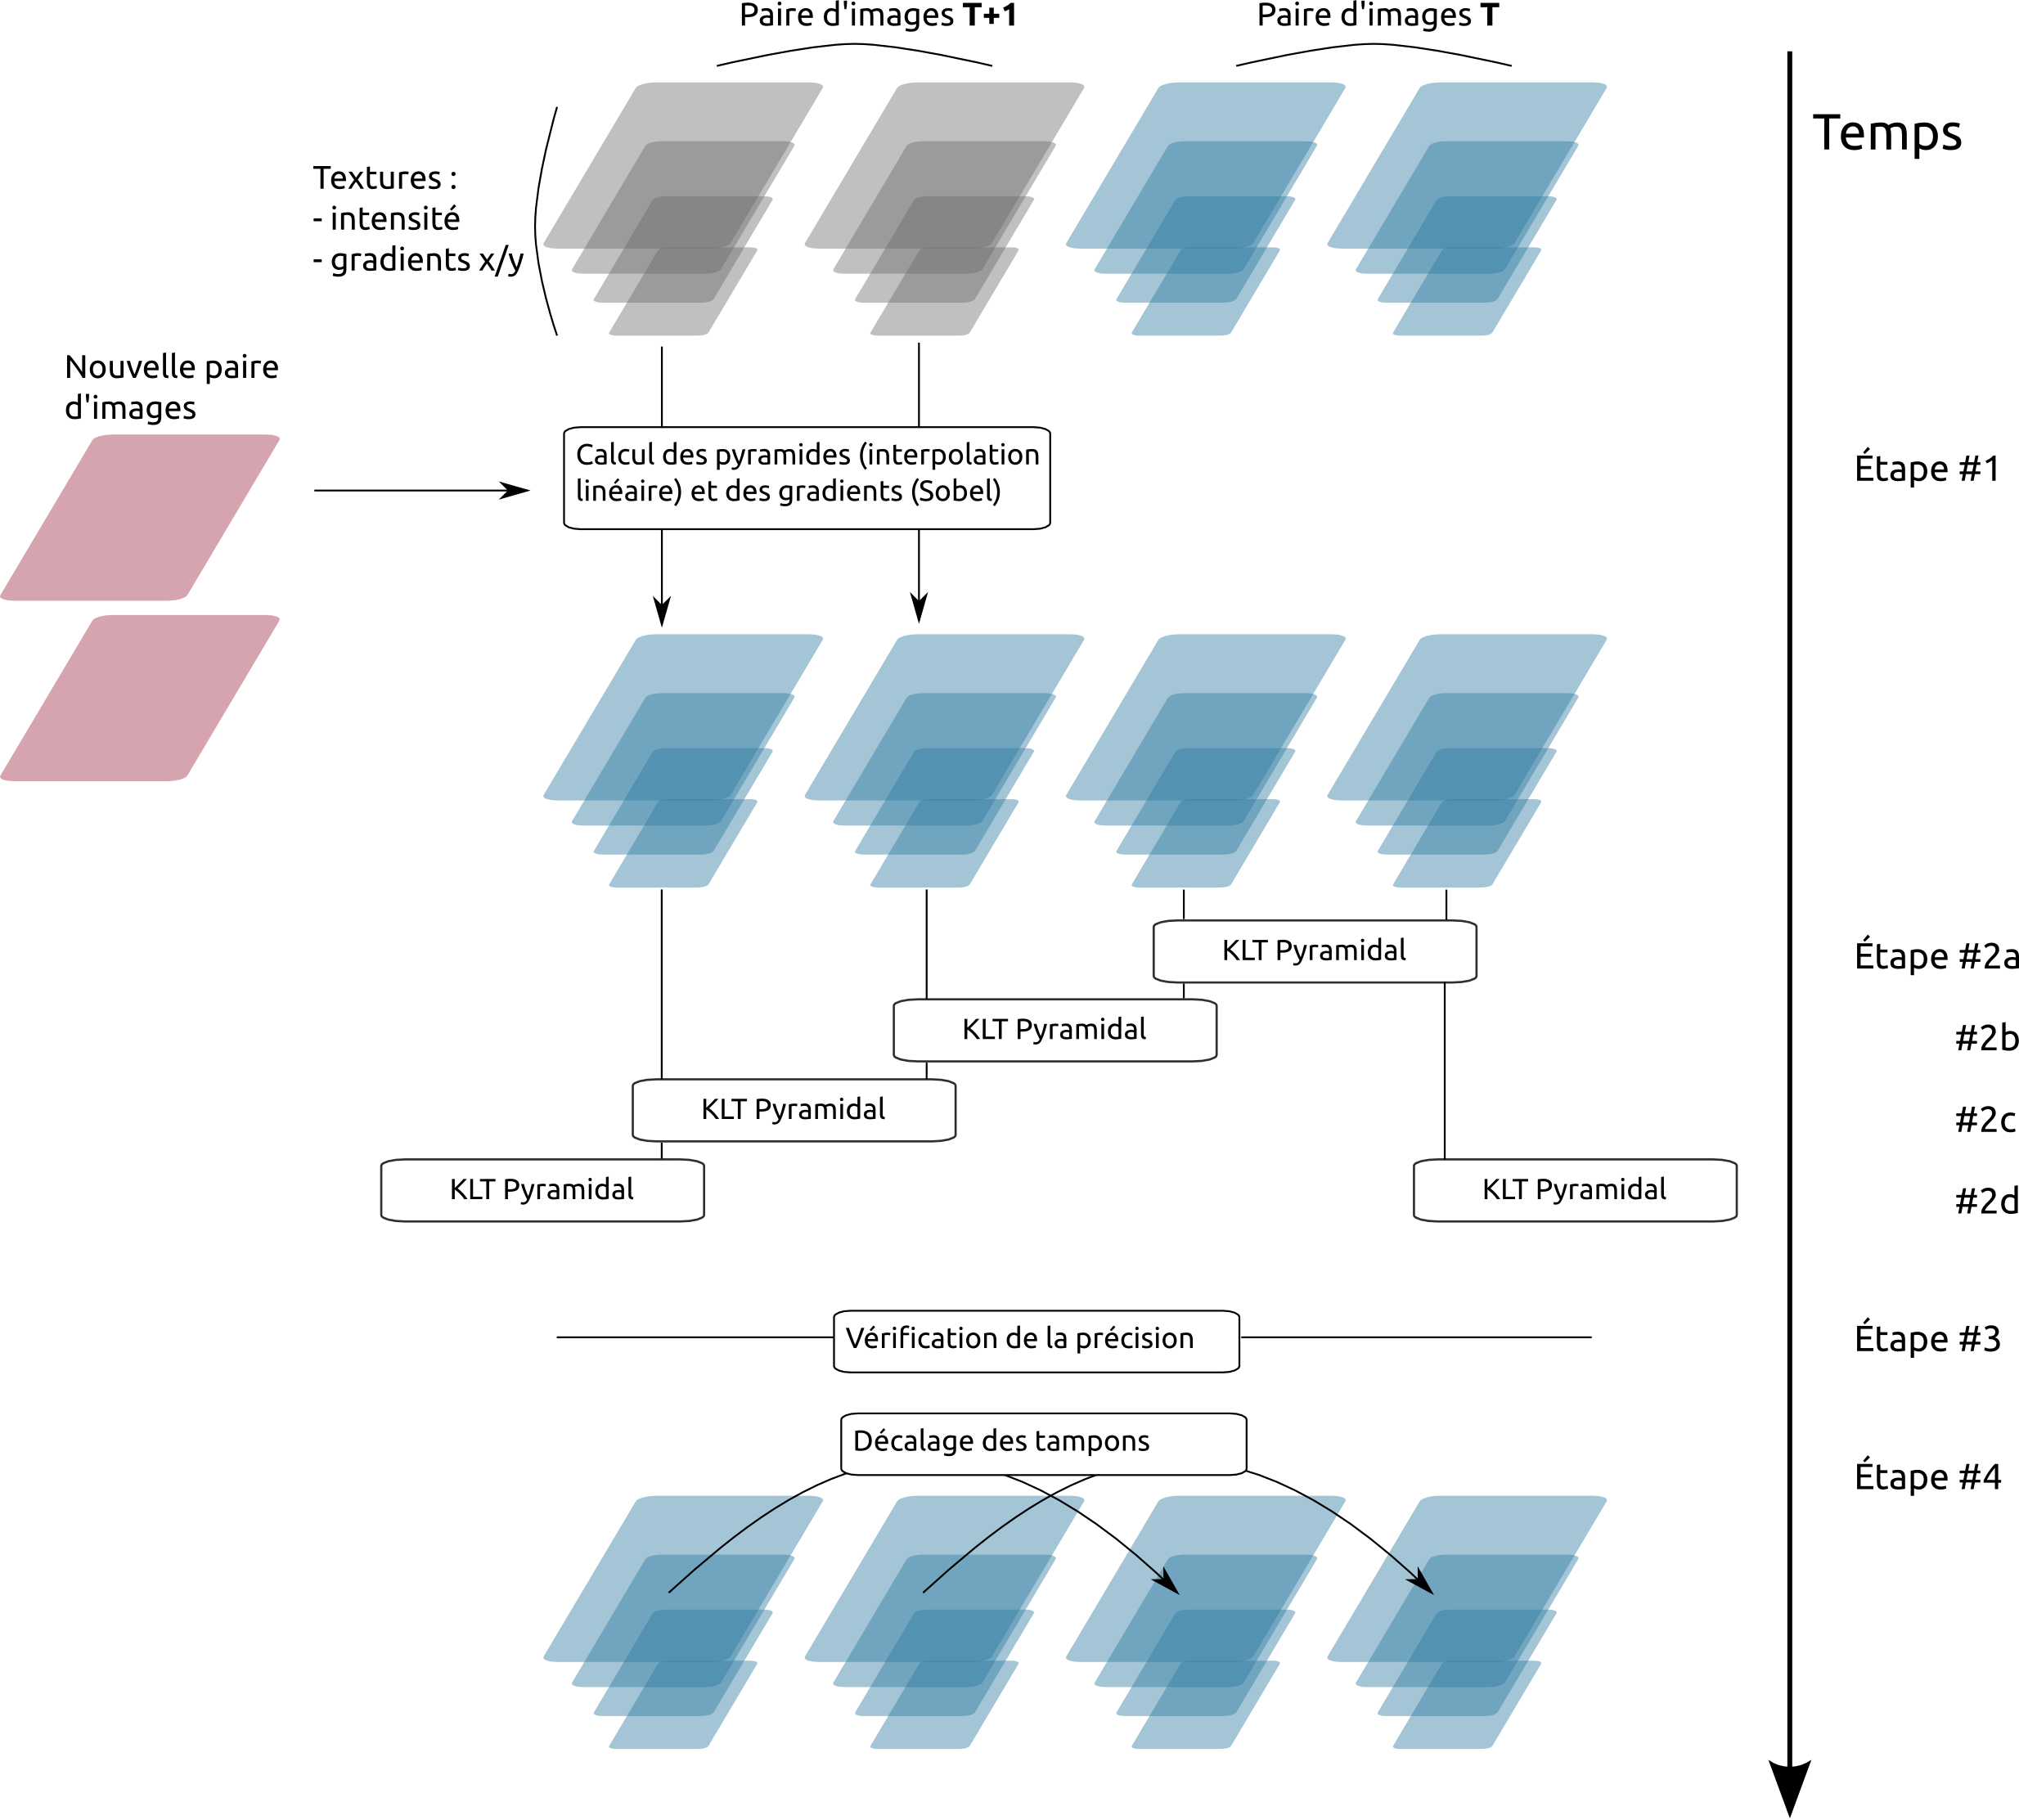
\includegraphics[width=1.3\textwidth]{Chapter3/graphics/4_Frames_implementation_diagram.png}
	}
	\caption{Vue d'ensemble de l'implémentation proposée pour un suivi redondant de points sur GPU. L'axe horizontal correspond à une exécution en parallèle, l'axe vertical correspond à une exécution séquentielle.}
	\label{fig:ch3_GPU_KLT}	
\end{figure}

\subsubsection{Comparaison : CPU/GPU}
Les performances en termes de robustesse et qualité du suivi sont équivalentes entre les différentes implémentations, comme attendu (s'agissant d'une application directe de \cite{Bouguet2001a} dans tous les cas). L'évaluation du temps de calcul est rendue délicate par sa dépendance à la plate-forme utilisée. On compare dans le tableau \ref{tab:ch3_comp_cpu_gpu} les performances obtenues par différents circuits présents dans le commerce, qui sont cependant en deçà de l'état de l'art en la matière (la GTX470 est sortie en 2010). Il s'agit donc de performances aisément accessibles en 2013, et un suivi de points plus ambitieux (quasi-dense) est sans doute possible. Le temps de calcul présenté vaut pour 4000 points, une taille d'image de 512 x 384, 5 étages de pyramide et un voisinage de 7x7 pixels. On note \emph{4Frame} notre implémentation purement CUDA conçue autour du suivi redondant sur 4 images. L'implémentation OpenCV-GPU présentée n'est pas spécialement optimisée pour notre tâche, il est sans doute possible de faire un peu mieux sans toutefois - à notre avis - atteindre les performances d'une implémentation dédiée. La version 2.4 de la librairie OpenCV est utilisée.

\begin{table}[H]
	\centerline {
		\begin{tabular}{| c | c | c | c | c | c |} 
			\hline
			Méthode & Support & Processeur & \pbox{5cm}{Unités \\ d'exécution} & \pbox{5cm}{Temps de \\ calcul (ms)} & Framerate\\
			\hline
			OpenCV & CPU & Intel Core i7 	& 4 	& 43 	& 23\\
			\hline
			OpenCV & GPU & nVidia GTX470	& 448 &	70 	& 14	\\
			\hline
			OpenCV & GPU & nVidia GTX460m & 192	& 115 & 9		\\
			\hline
			\textit{4Frame} & GPU & nVidia GTX470 	& 448 &\textbf{27} 	& \textbf{37}	\\
			\hline
			\textit{4Frame} & GPU & nVidia GTX460m & 192 & 42 	& 23	\\
			\hline
		\end{tabular}
	}
	\caption{Comparaison des temps de calculs selon différentes méthodes et unités de calcul. 4000 points sont suivis de manière redondante.}
	\label{tab:ch3_comp_cpu_gpu}
\end{table}

On pourra tout d'abord remarquer que le gain en performances attendu par une implémentation massivement parallèle (la GTX 470 dispose de 448 unités d'exécution, la GTX460m de 192 unités, contre 4 unités pour le CPU considéré) n'est pas directement observé en pratique. Les unités de calcul de type \og CPU\fg{} et \og GPU\fg{} ne sont tout d'abord par directement comparables, même si le nombre de processus exécutés simultanément est effectivement de l'ordre du nombre d'unités annoncées. Il est possible d'obtenir des performances significativement améliorées par l'implémentation très parallélisée, mais le caractère un peu aléatoire de la position des points à suivre est préjudiciable au cadre SIMD (\emph{Single Instruction Multiple Data} - Instruction Unique, Données Multiples) imposé par les GPU. Le facteur limitant du temps d'exécution d'un programme est par ailleurs beaucoup plus complexe que le seul nombre d'unités qui lui sont consacrées. \\

On pourra ensuite constater qu'une implémentation \og naïve\fg{} sur GPU n'est pas vraiment profitable dans cette application. Ceci peut s'expliquer par des transferts inutiles entre les espaces mémoire CPU/GPU, et par des tâches répétitives dans le cycle de suivi de point qui ne sont pas exploitées. On rejoint en cela une remarque précédente, signalant la grande disparité de performances possibles dans le cadre d'une implémentation massivement parallèle. On peut enfin remarquer que le gain obtenu entre les circuits \emph{470} et \emph{460m} est de l'ordre de 1.55, tandis que les unités d'exécution sont 2.3 fois plus importantes, ce qui laisse supposer que notre implémentation pourrait être améliorée.

\section{Conclusion}
On a présenté dans cette partie différentes méthodes de l'état de l'art pour extraire des informations à partir de flux d'images. Nous nous sommes concentrés sur le suivi de points singuliers dans une séquence d'images, bien que d'autres concepts puissent être mis en œuvre, et nous avons proposé un suivi de points redondant nous permettant d'évaluer en tout point la fiabilité du suivi. Une comparaison de différents algorithmes de détection de points d'intérêt nous a permis de sélectionner le détecteur de Shi et Tomasi comme étant le plus approprié pour notre application. Nous avons ensuite proposé une implémentation GPU du suivi redondant de points, et nous l'avons comparé à plusieurs implémentations de l'état de l'art. On peut finalement vérifier que le suivi fiable et en temps réel de plusieurs milliers de points est possible, ce qui nous amène à en proposer une exploitation dans le cadre de l'odométrie visuelle, de la reconstruction de l'environnement et de la détection d'objets mobiles.